\section{Performance Evaluation}
\label{sec:results}

In this section we describe the experimental evaluation of the algorithm proposed, including the scenarios, metrics, methodology and outcomes.


\subsection{QoE Metric evaluation}

There exist many viewer QoE models in the literature. we will describe the QoE metrics used to score the user satisfaction. Firstly, We compute each video quality chunk by a logarithmic law over bit-rates. Study in [11] propose a video quality model for DASH as shown in Equation (1). Each video has $N$ chunks and is encoded with $L$ bitrate levels. $r_i$ represents a specific bitrate level. At each step $i$, the quality of chunk $i$ which is encoded at $l_i$ is defined as:

$$
q(r_i) = a_1 * log(a_2 * (r_i/ r_{|L|}))
$$

To quantify a long-term users' QoE, we require a flexible QoE model that includes the most effective metrics. 
We consider the Eqn. (7) which consists of four metrics: (a) the average chunk perceptual quality, (b) the average number of quality oscillations, (c) the average number of stall events and their durations, and (d) the startup delay. K

\begin{equation}\label{qoe-equation}
QoE_i = \alpha_1 + \alpha_2 + \alpha_3 + \alpha_4
\end{equation}


The QoE has a range of 1 to 5. Where the values 1 = bad, 2 = poor, 3 = fair, 4 = good, and 5 = excellent.
 
\subsection{Experimental Setup}

%[29] Christian Kreuzberger, Daniel Posch, and Hermann Hellwagner. Amust framework - adaptive multimedia streaming simulation framework for ns-3 and ndnsim, 2016.
%[30] C. Mueller, S. Lederer, J. Poecher, and C. Timmerer. Demo paper: Libdash - an open source software library for the mpeg-dash standard. In 2013 IEEE International Conference on Multimedia and Expo Workshops (ICMEW), pages 1–2, July 2013.
% Per-title encode optimization, 2015. ; accessed 20-novembro-2019.

To implement DASH servers and users that allow adaptive video streaming, we use Adaptive Multimedia Streaming~(AMuSt)~[1]. The AMuSt framework provides a set of applications for producing and consuming adaptable video, based on the DASH standard. DASH functionality is provided by the libdash library~[2], an open source library that provides an interface to the DASH standard. Currently, libdash is the official reference software for the DASH standard. We consider that users are interested in an available video with ten different bit rate representations \{235kbps, 375kbps, 560kbps, 560kbps, 750kbps, 1050kbps, 1750kbps, 2350kbps, 3000kbps, 4300kbps, 5800kbps\}, which are used by Netflix subsets~[3], which are used by Netflix. [31]. Each representation is divided into 2-second segments. Each experiment was performed 10 times with an execution time of 1600 seconds. Figure 3 shows the topology with three levels used in the experiments, each level \{1, 2 and 3\} is represented as a scenario.


For sake of siplicity, the cache video userd in simulation are cosidered deployed in the edge dash nodes. 

Dash server and the clients allowed to request a multimedia content in DASH format, was used the Adaptive Multimedia Streaming~(AMuSt). The AMust system allow a set o apps to produce and consume the adaptive video, based on Dash pattern. The DASH functionality is provided by the libdash library, an open source library that provides an interface to the DASH standard. Currently, libdash is the reference software official DASH standard.

We simulate the scenario in a binary tree topology of height two.  Firstly, We compare with the cloud-only scenario, without edge server, to the difference with and without the edge use. 



% \begin{figure*}
%     \centering
%     \subfigure[]{
%     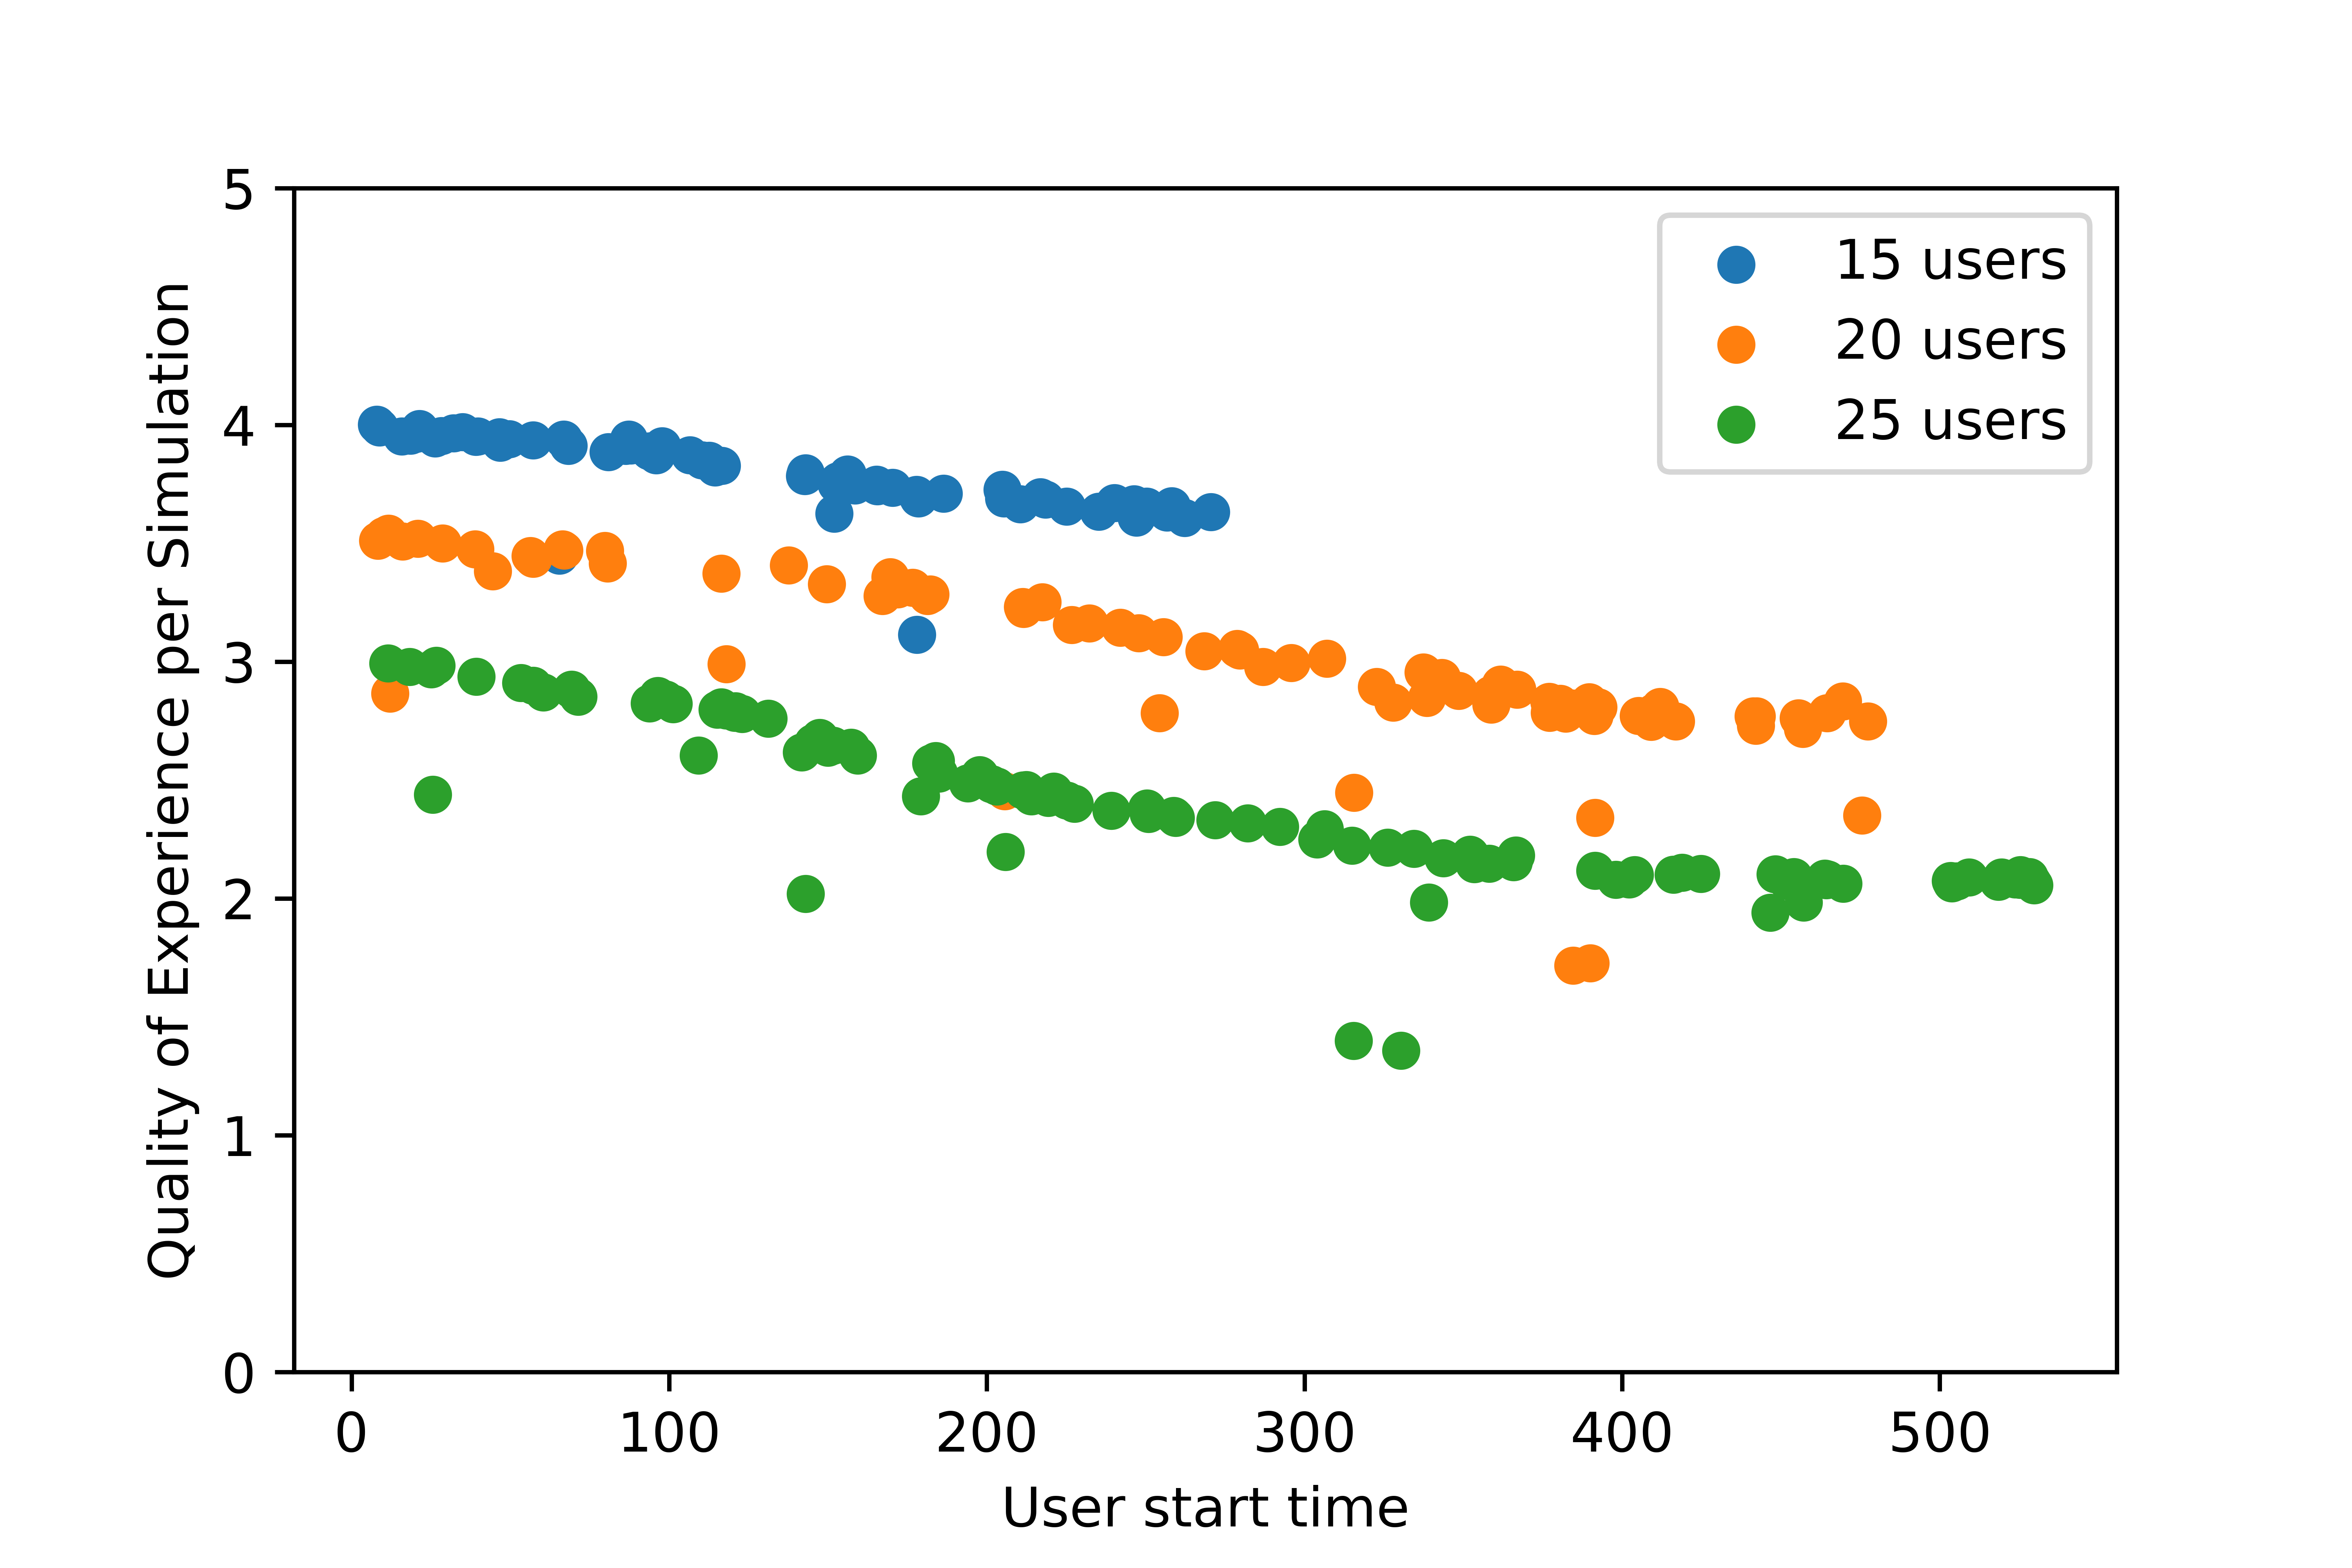
\includegraphics[width=0.45\linewidth]{images/QoECompare.png}
%     \label{fig:red-comparison-plot}
%     }
%     \subfigure[]{
%     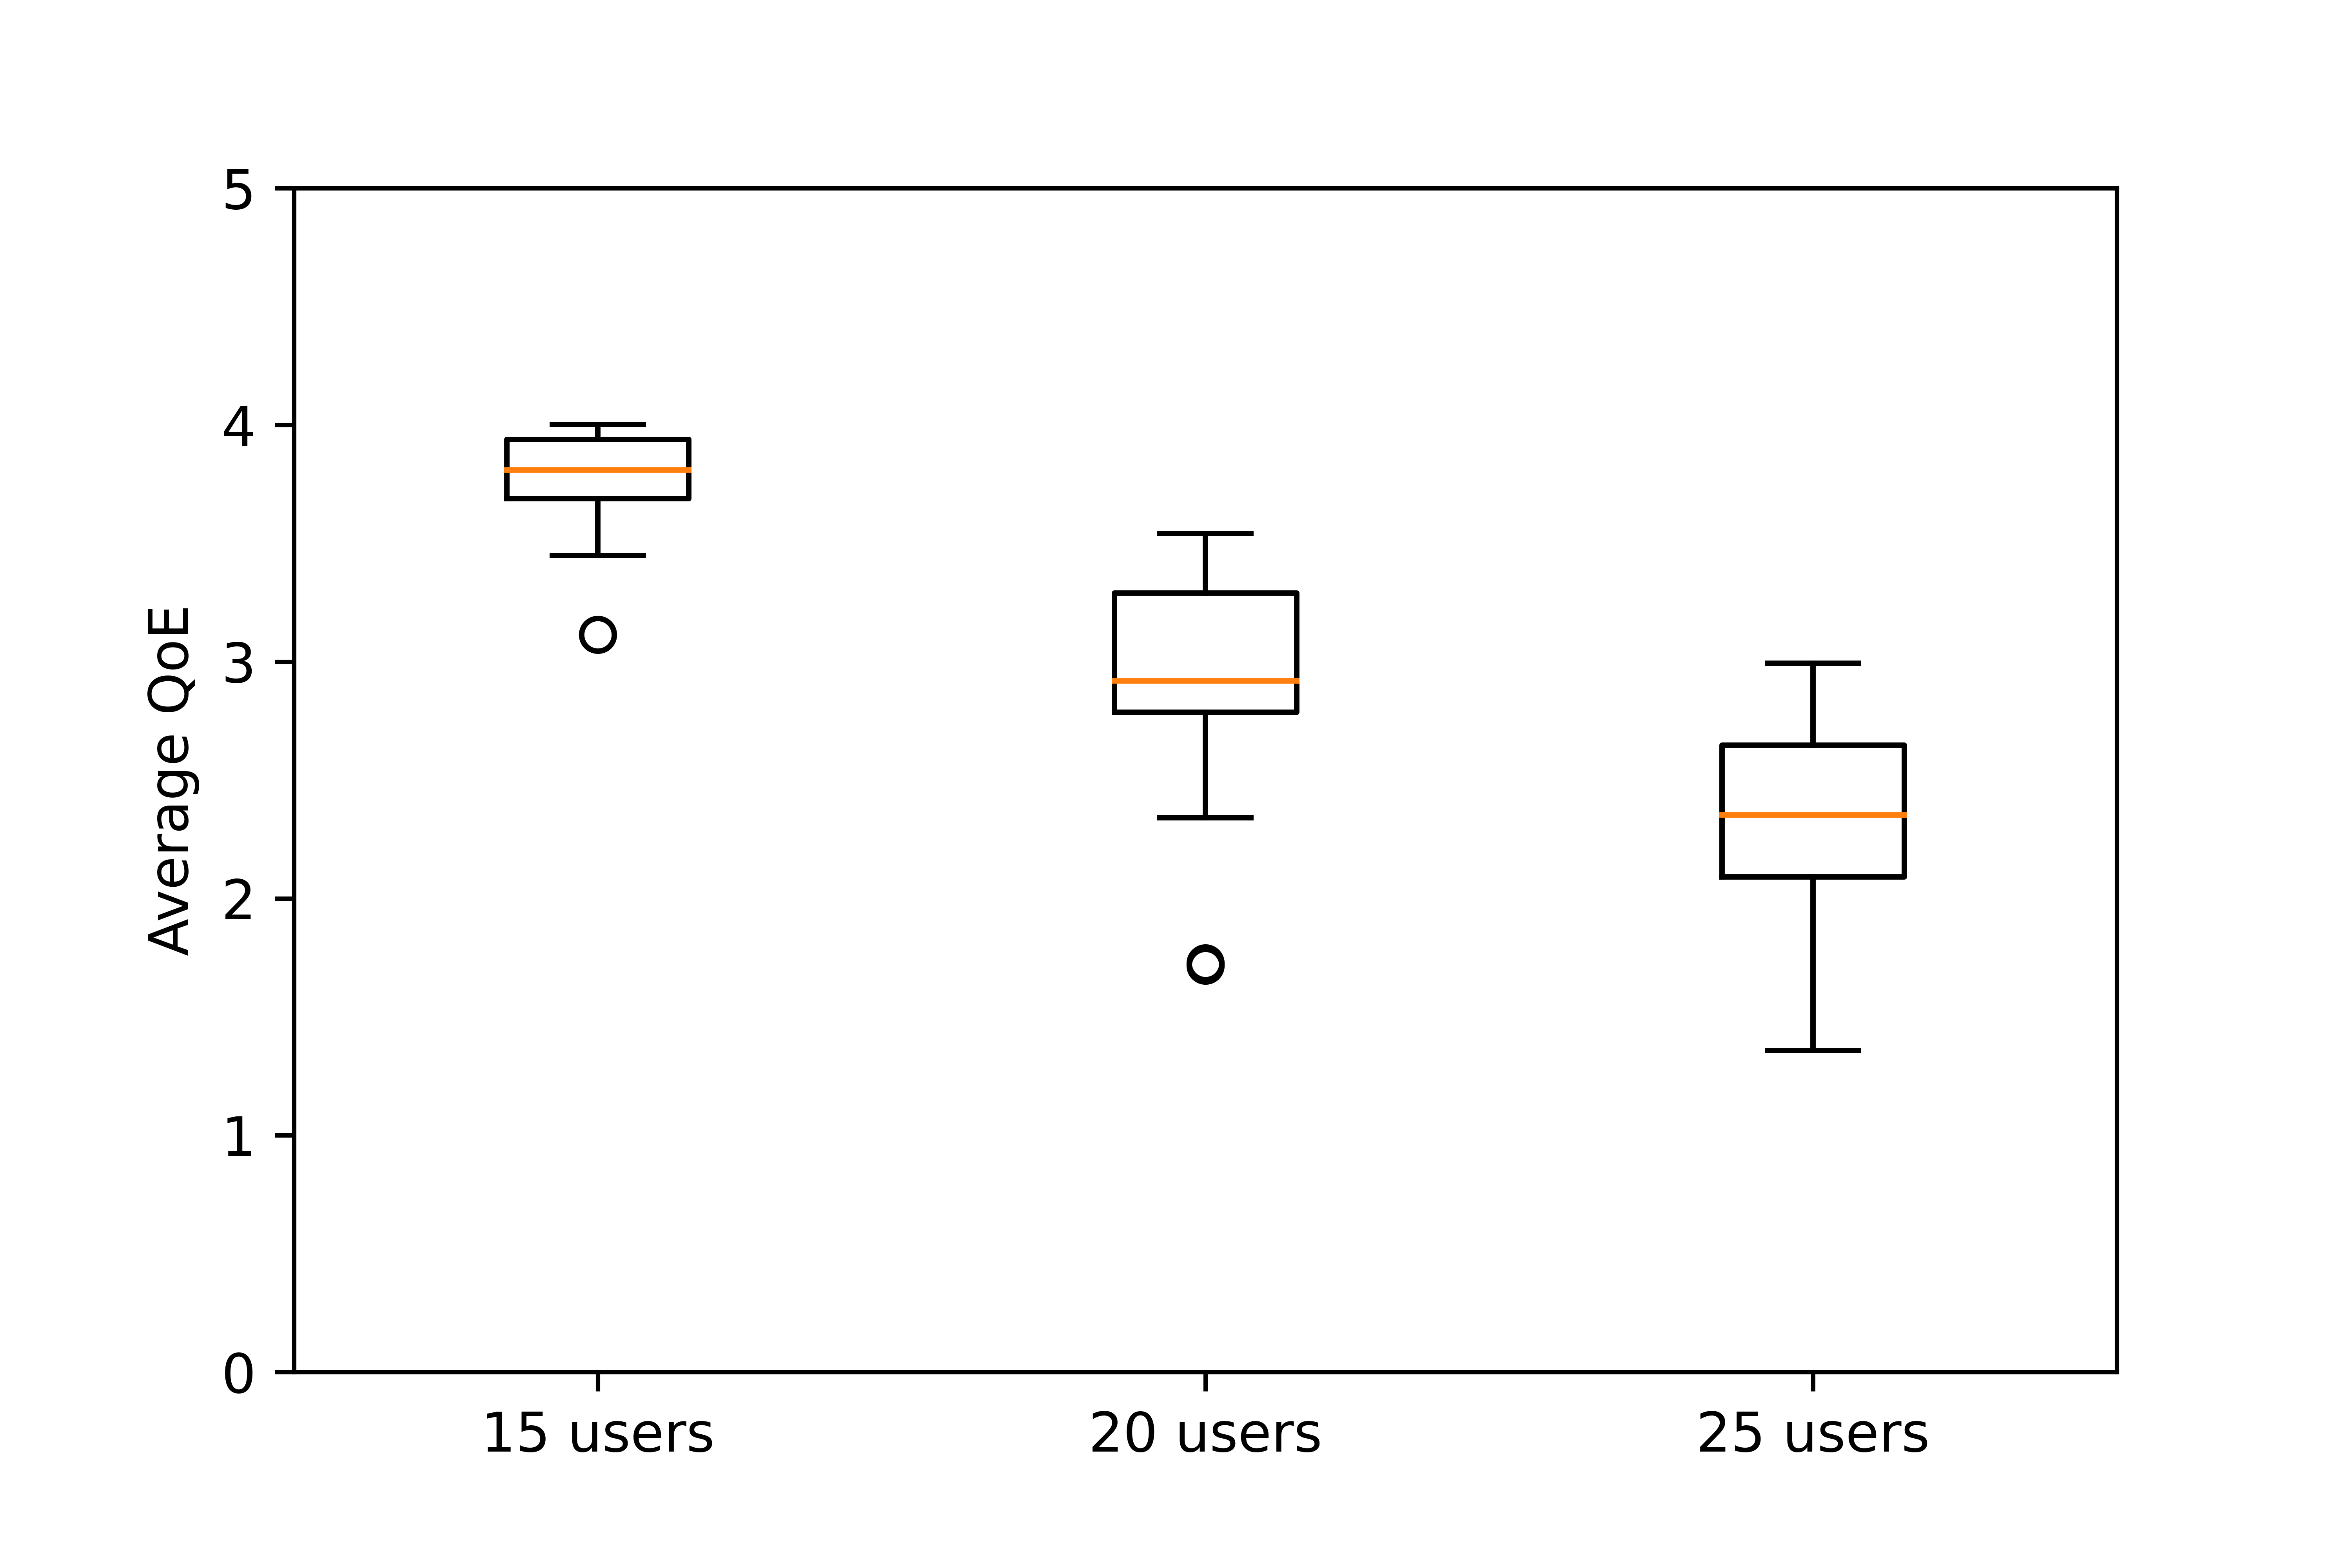
\includegraphics[width=0.45\linewidth]{images/QoEBoxplot.png}
%     \label{fig:co-comparison-boxplot}
%     }

%     \subfigure[]{
%     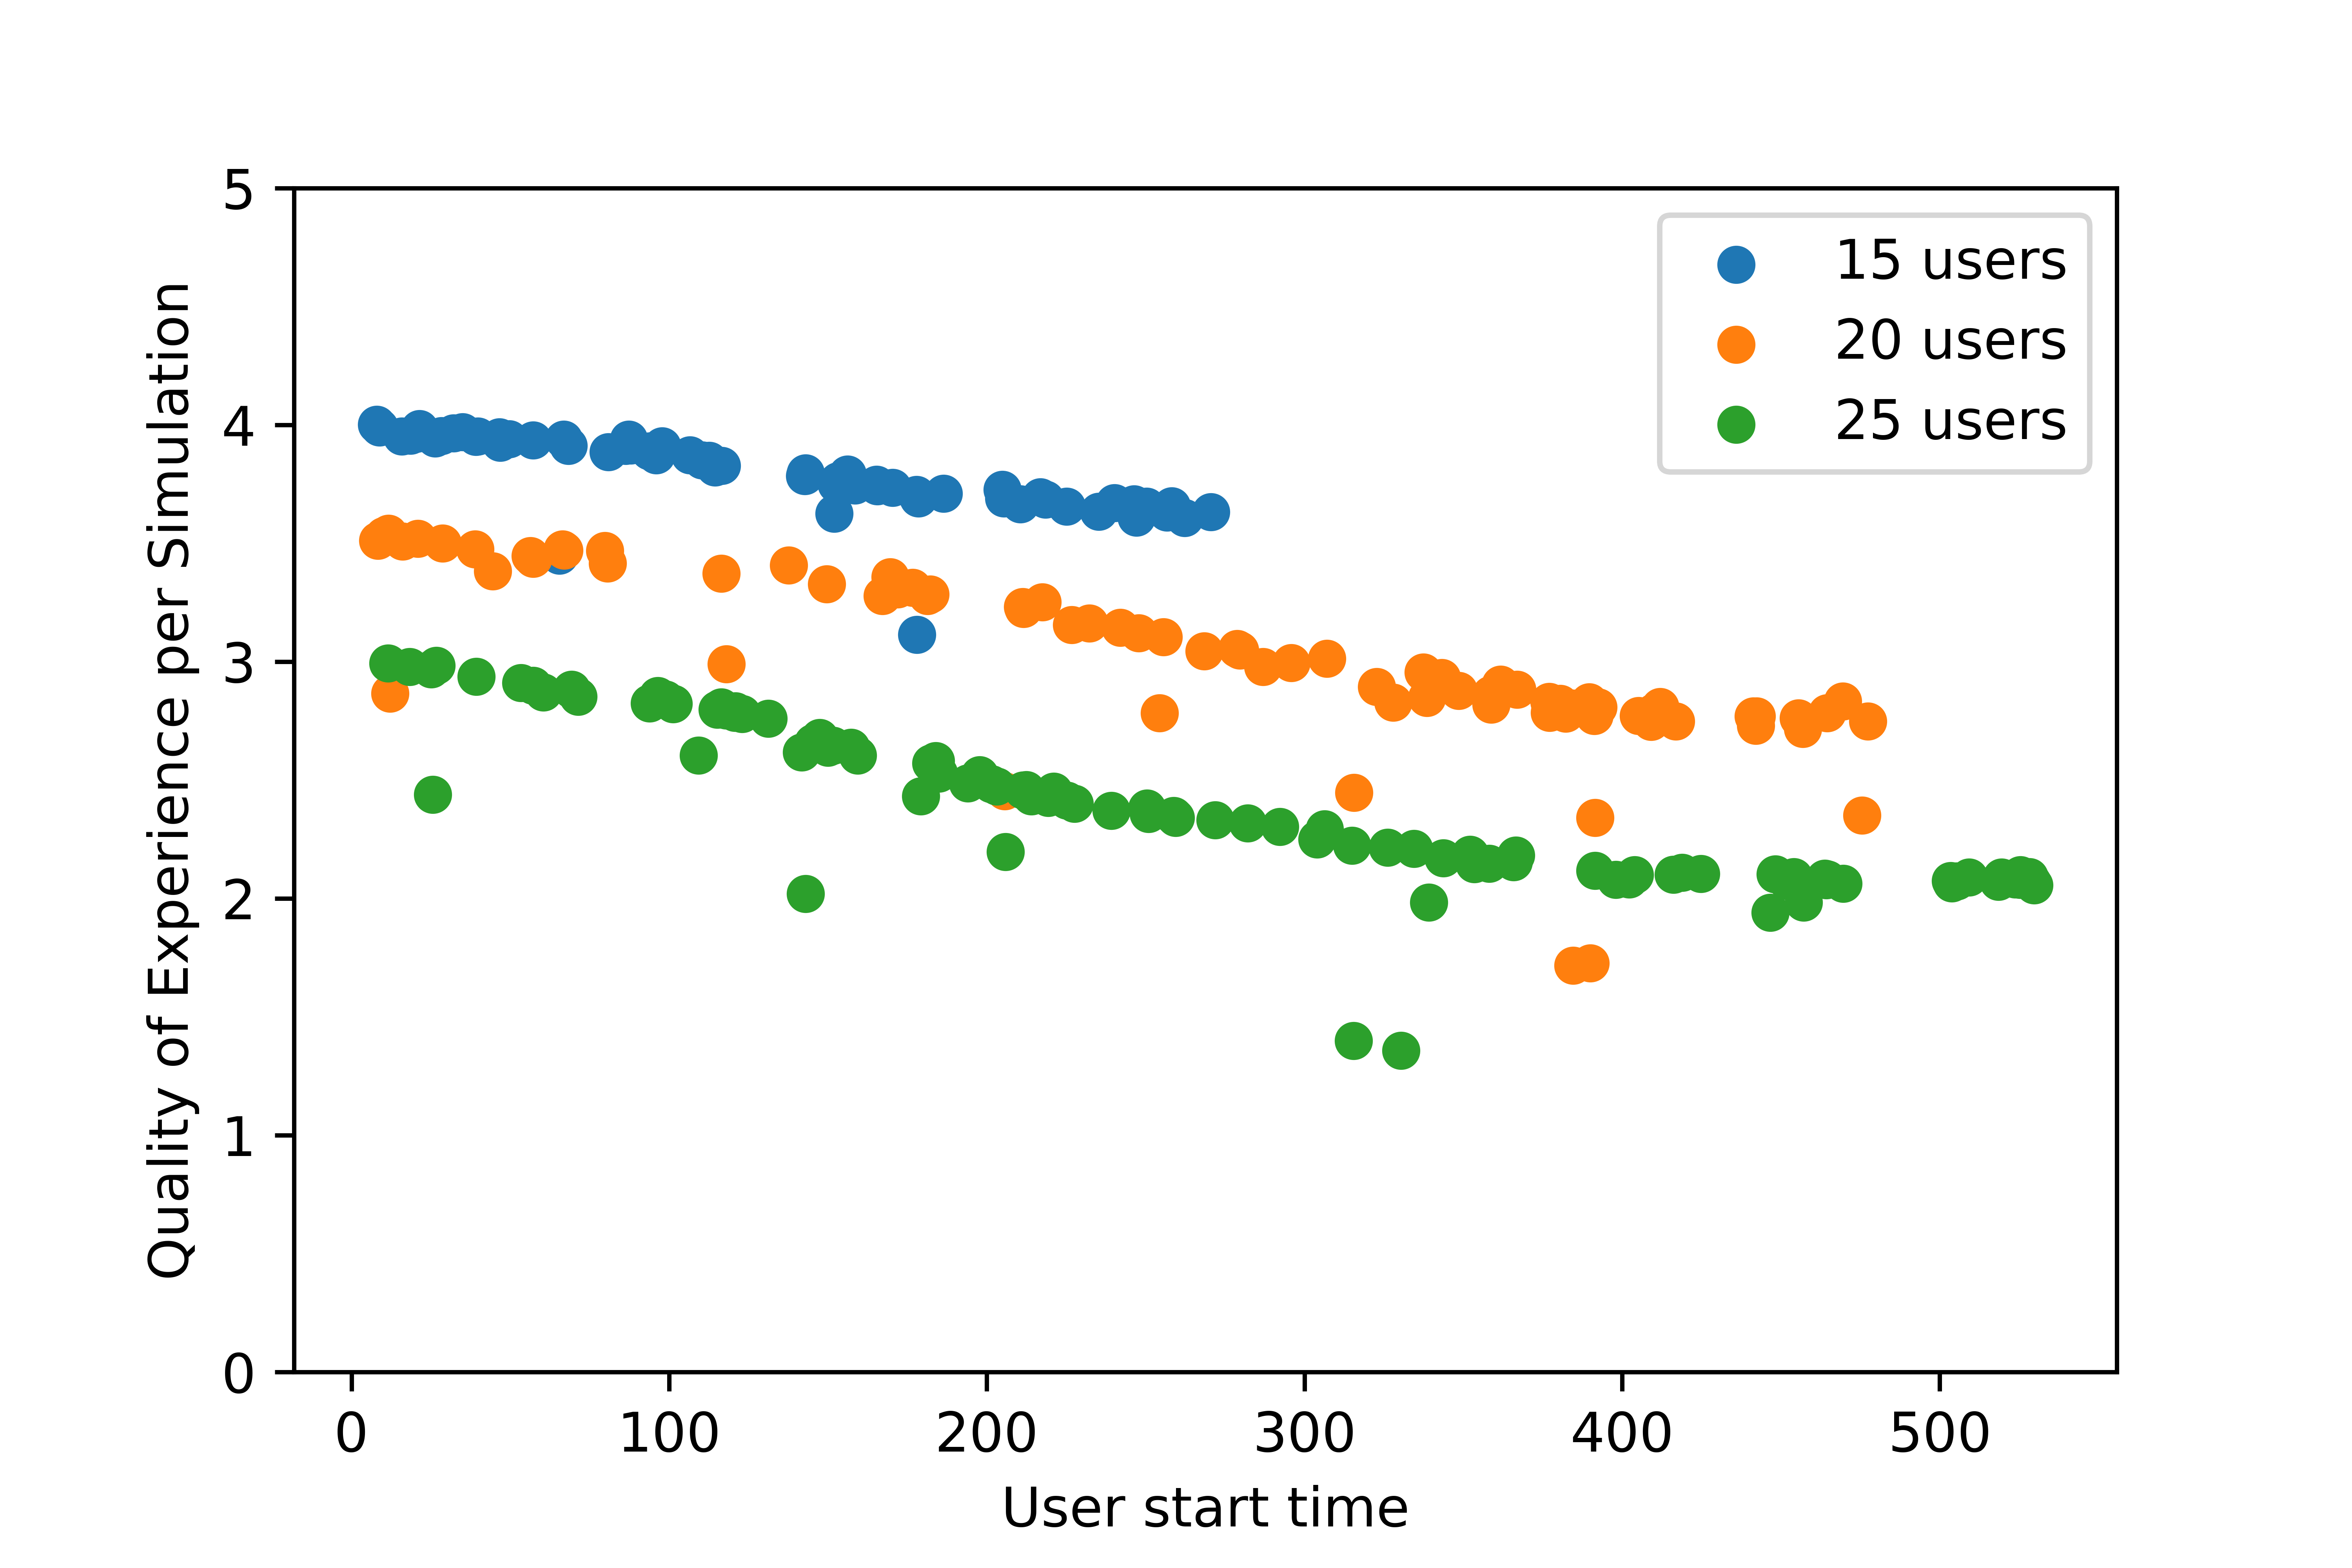
\includegraphics[width=0.45\linewidth]{images/QoECompare.png}
%     \label{fig:red-comparison-plot}
%     }
%     \subfigure[]{
%     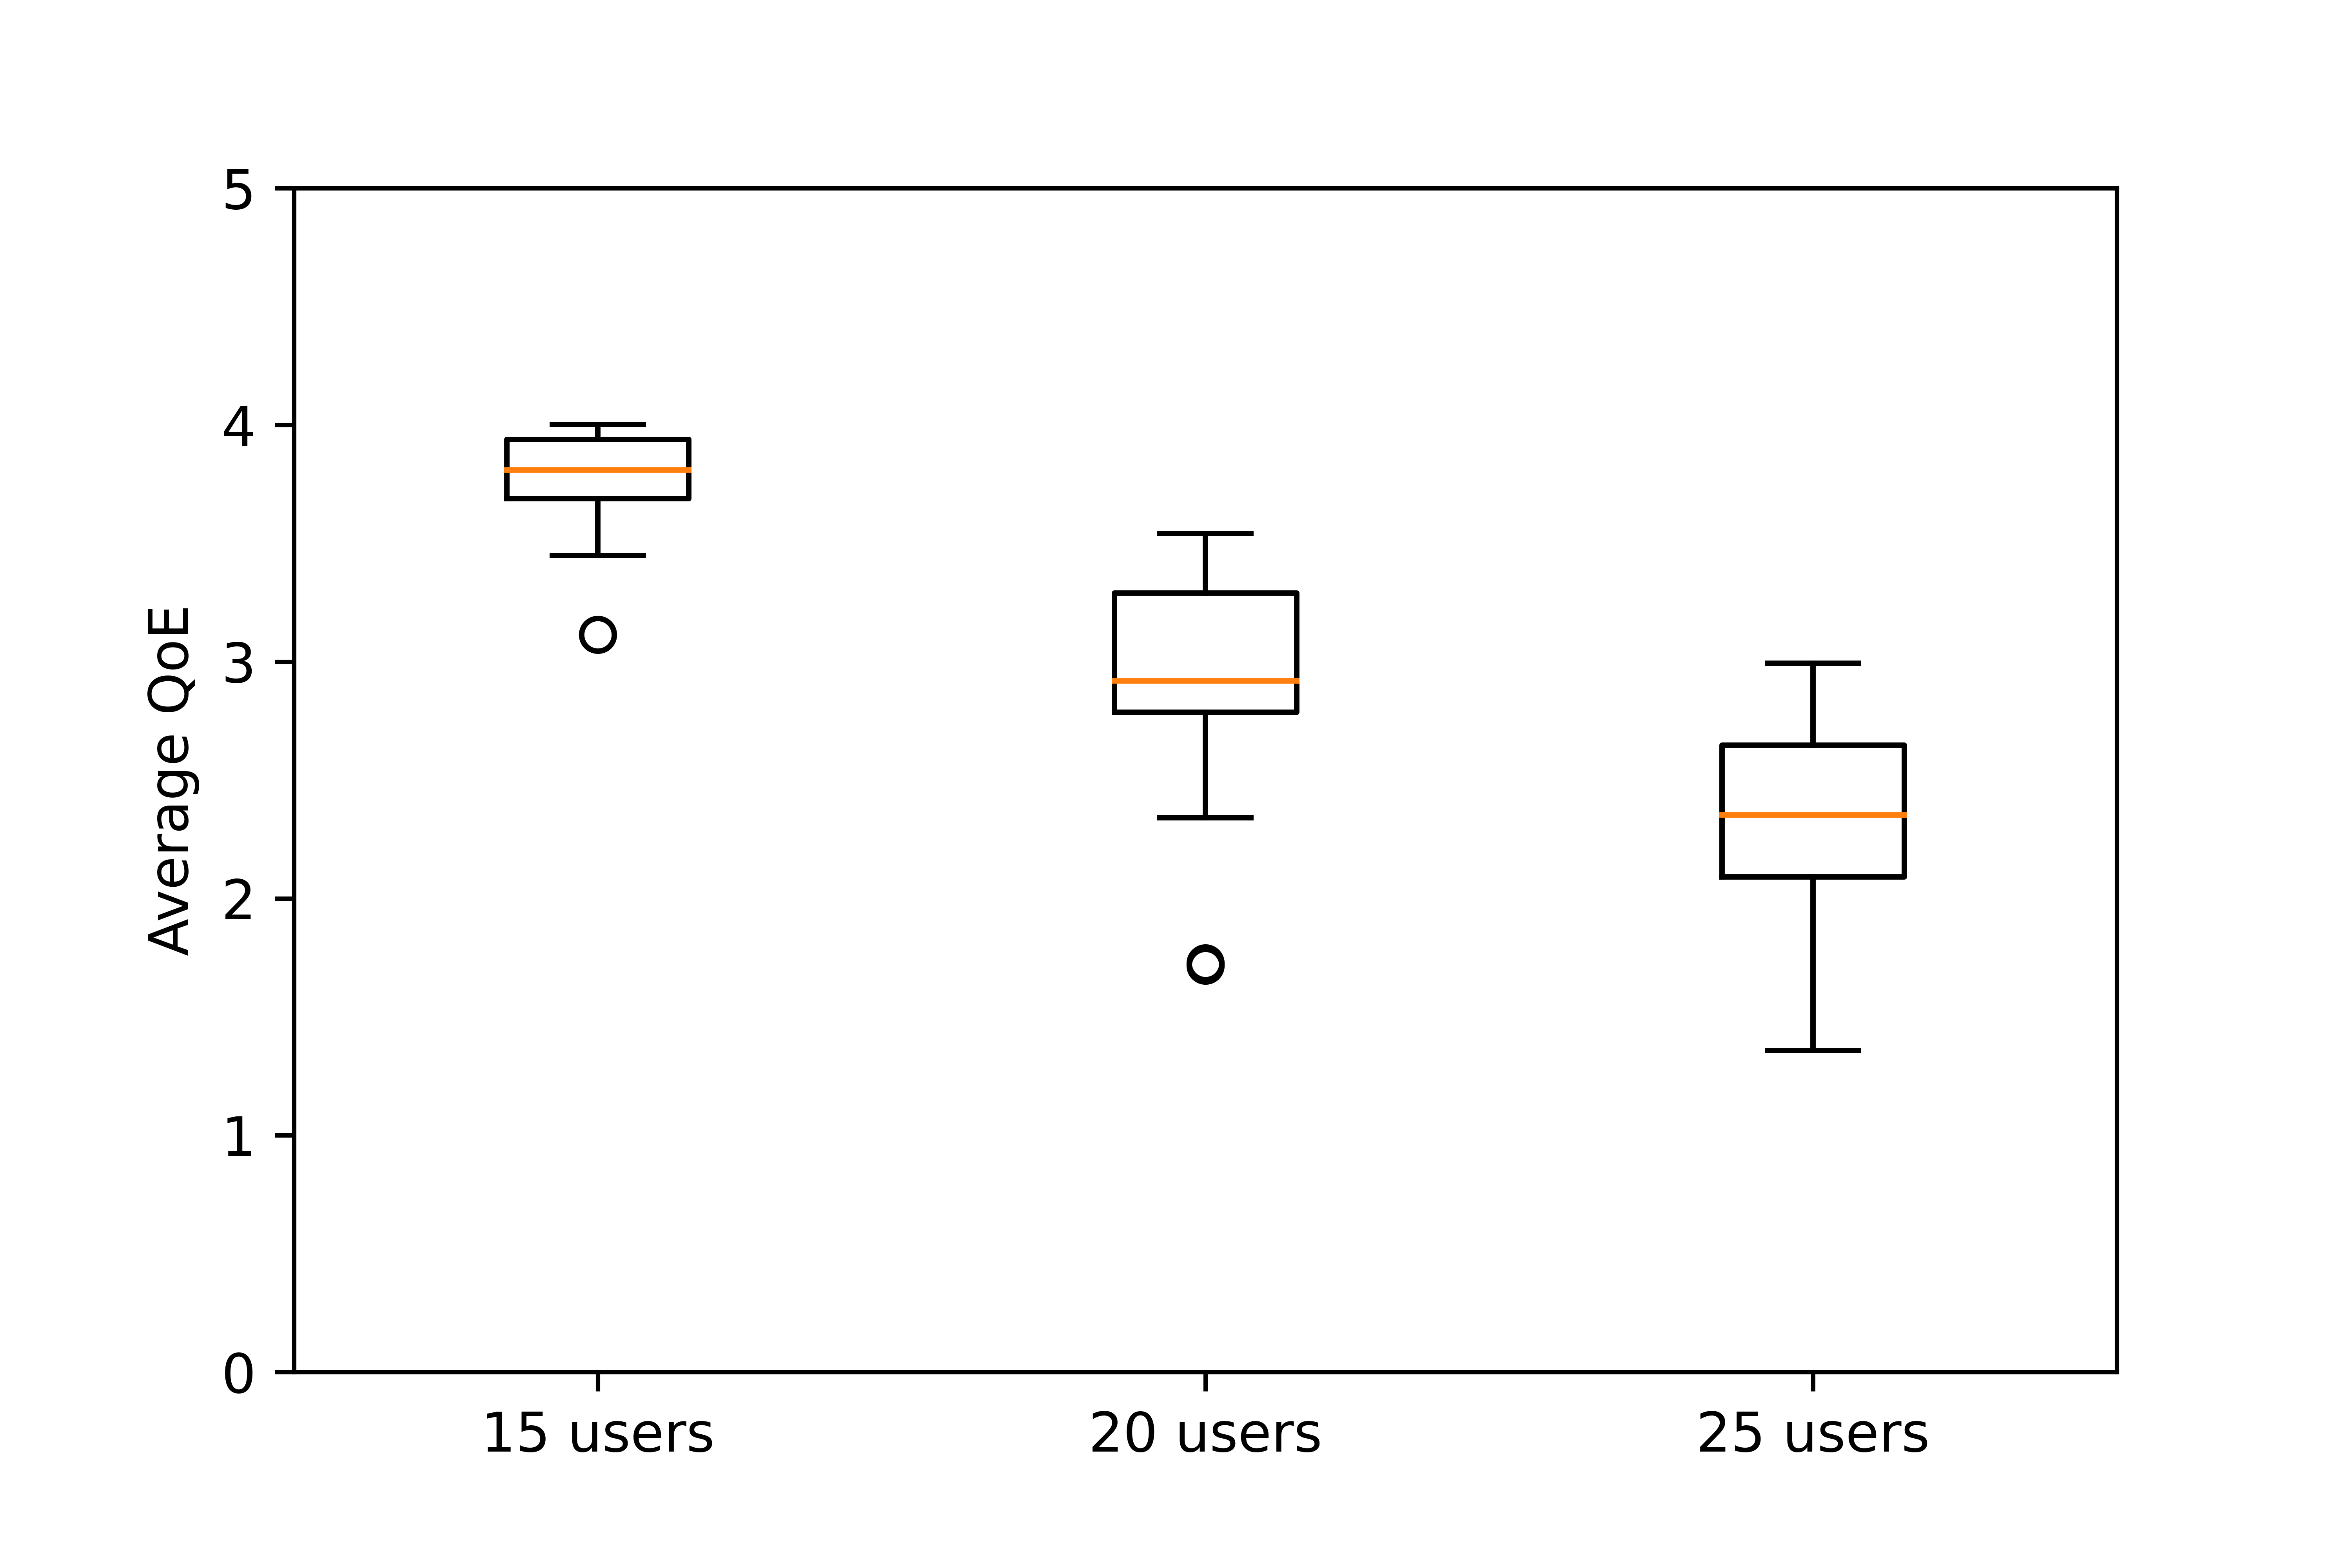
\includegraphics[width=0.45\linewidth]{images/QoEBoxplot.png}
%     \label{fig:red-comparison-boxplot}
%     }

%     \caption{Impact of system on the network performance. Distance \textit{d} between sensor node and antennas of 8m in a semi-NLOS scenario.}
%     \label{fig:comparison-rof-2}
% \end{figure*}

\begin{figure*}
    \centering
    \subfigure[]{
    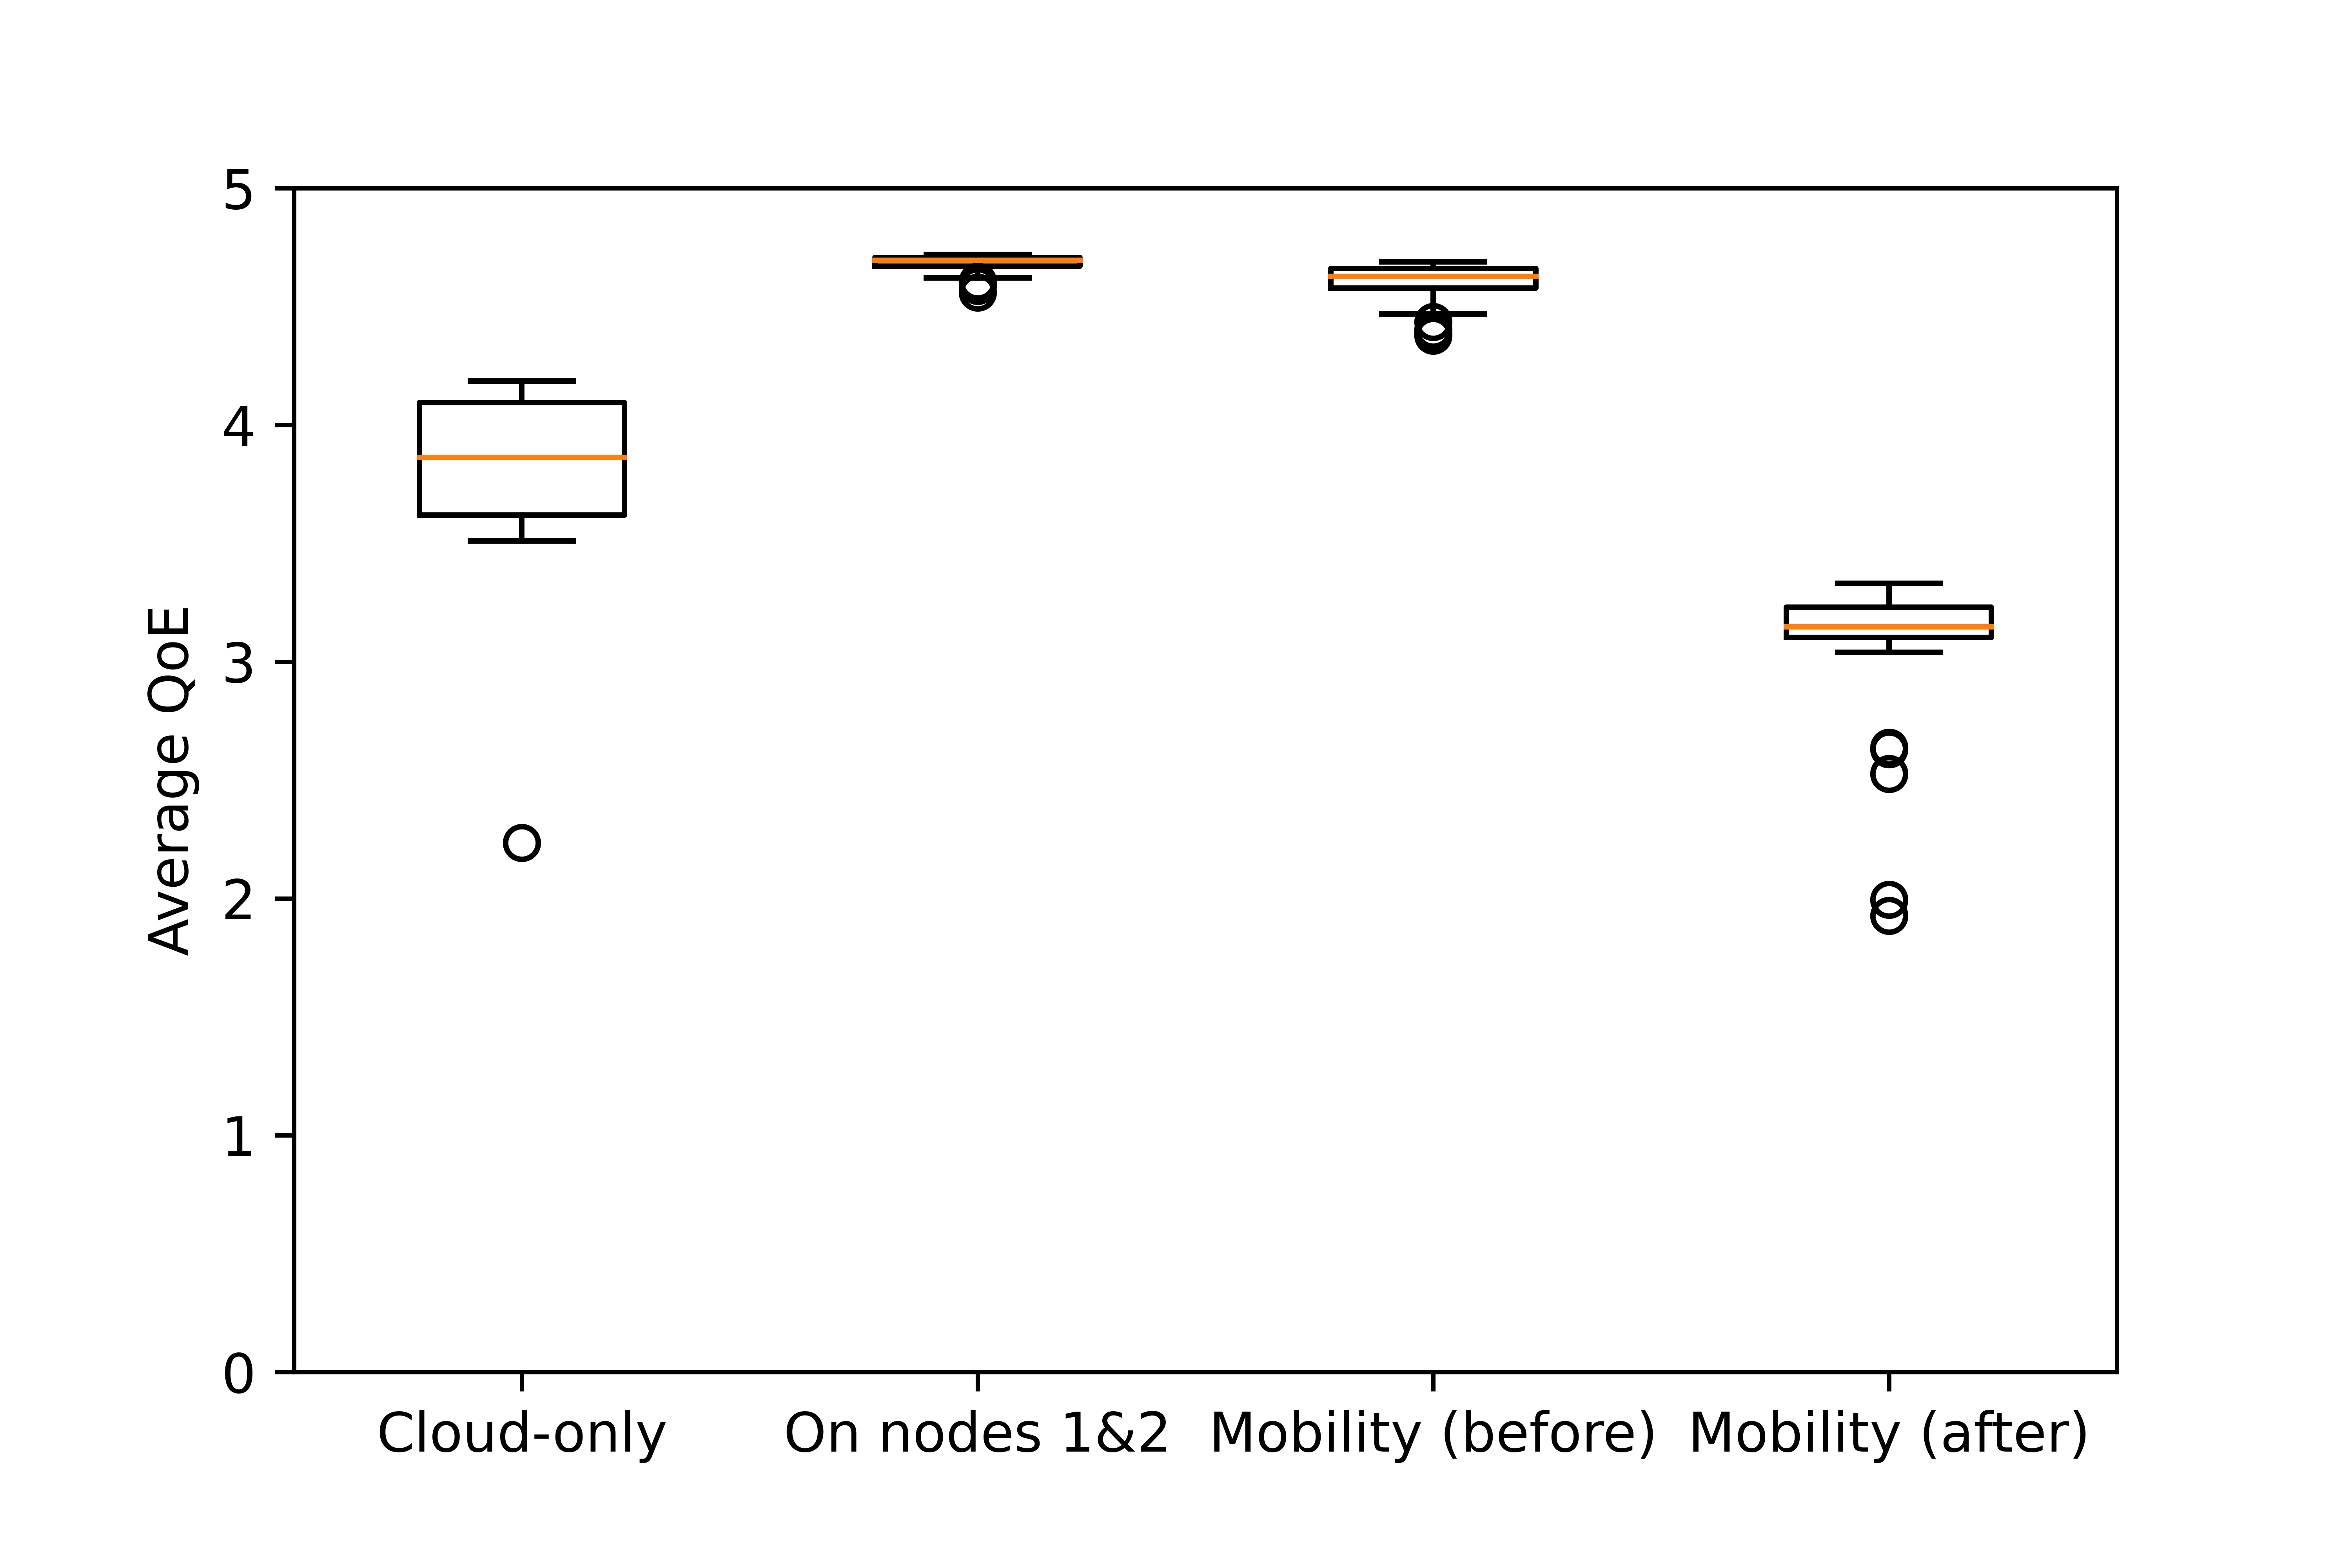
\includegraphics[width=0.31\linewidth]{images/QoEBoxplot-15u.png}
    \label{fig:red-comparison-plot}
    }
    \subfigure[]{
    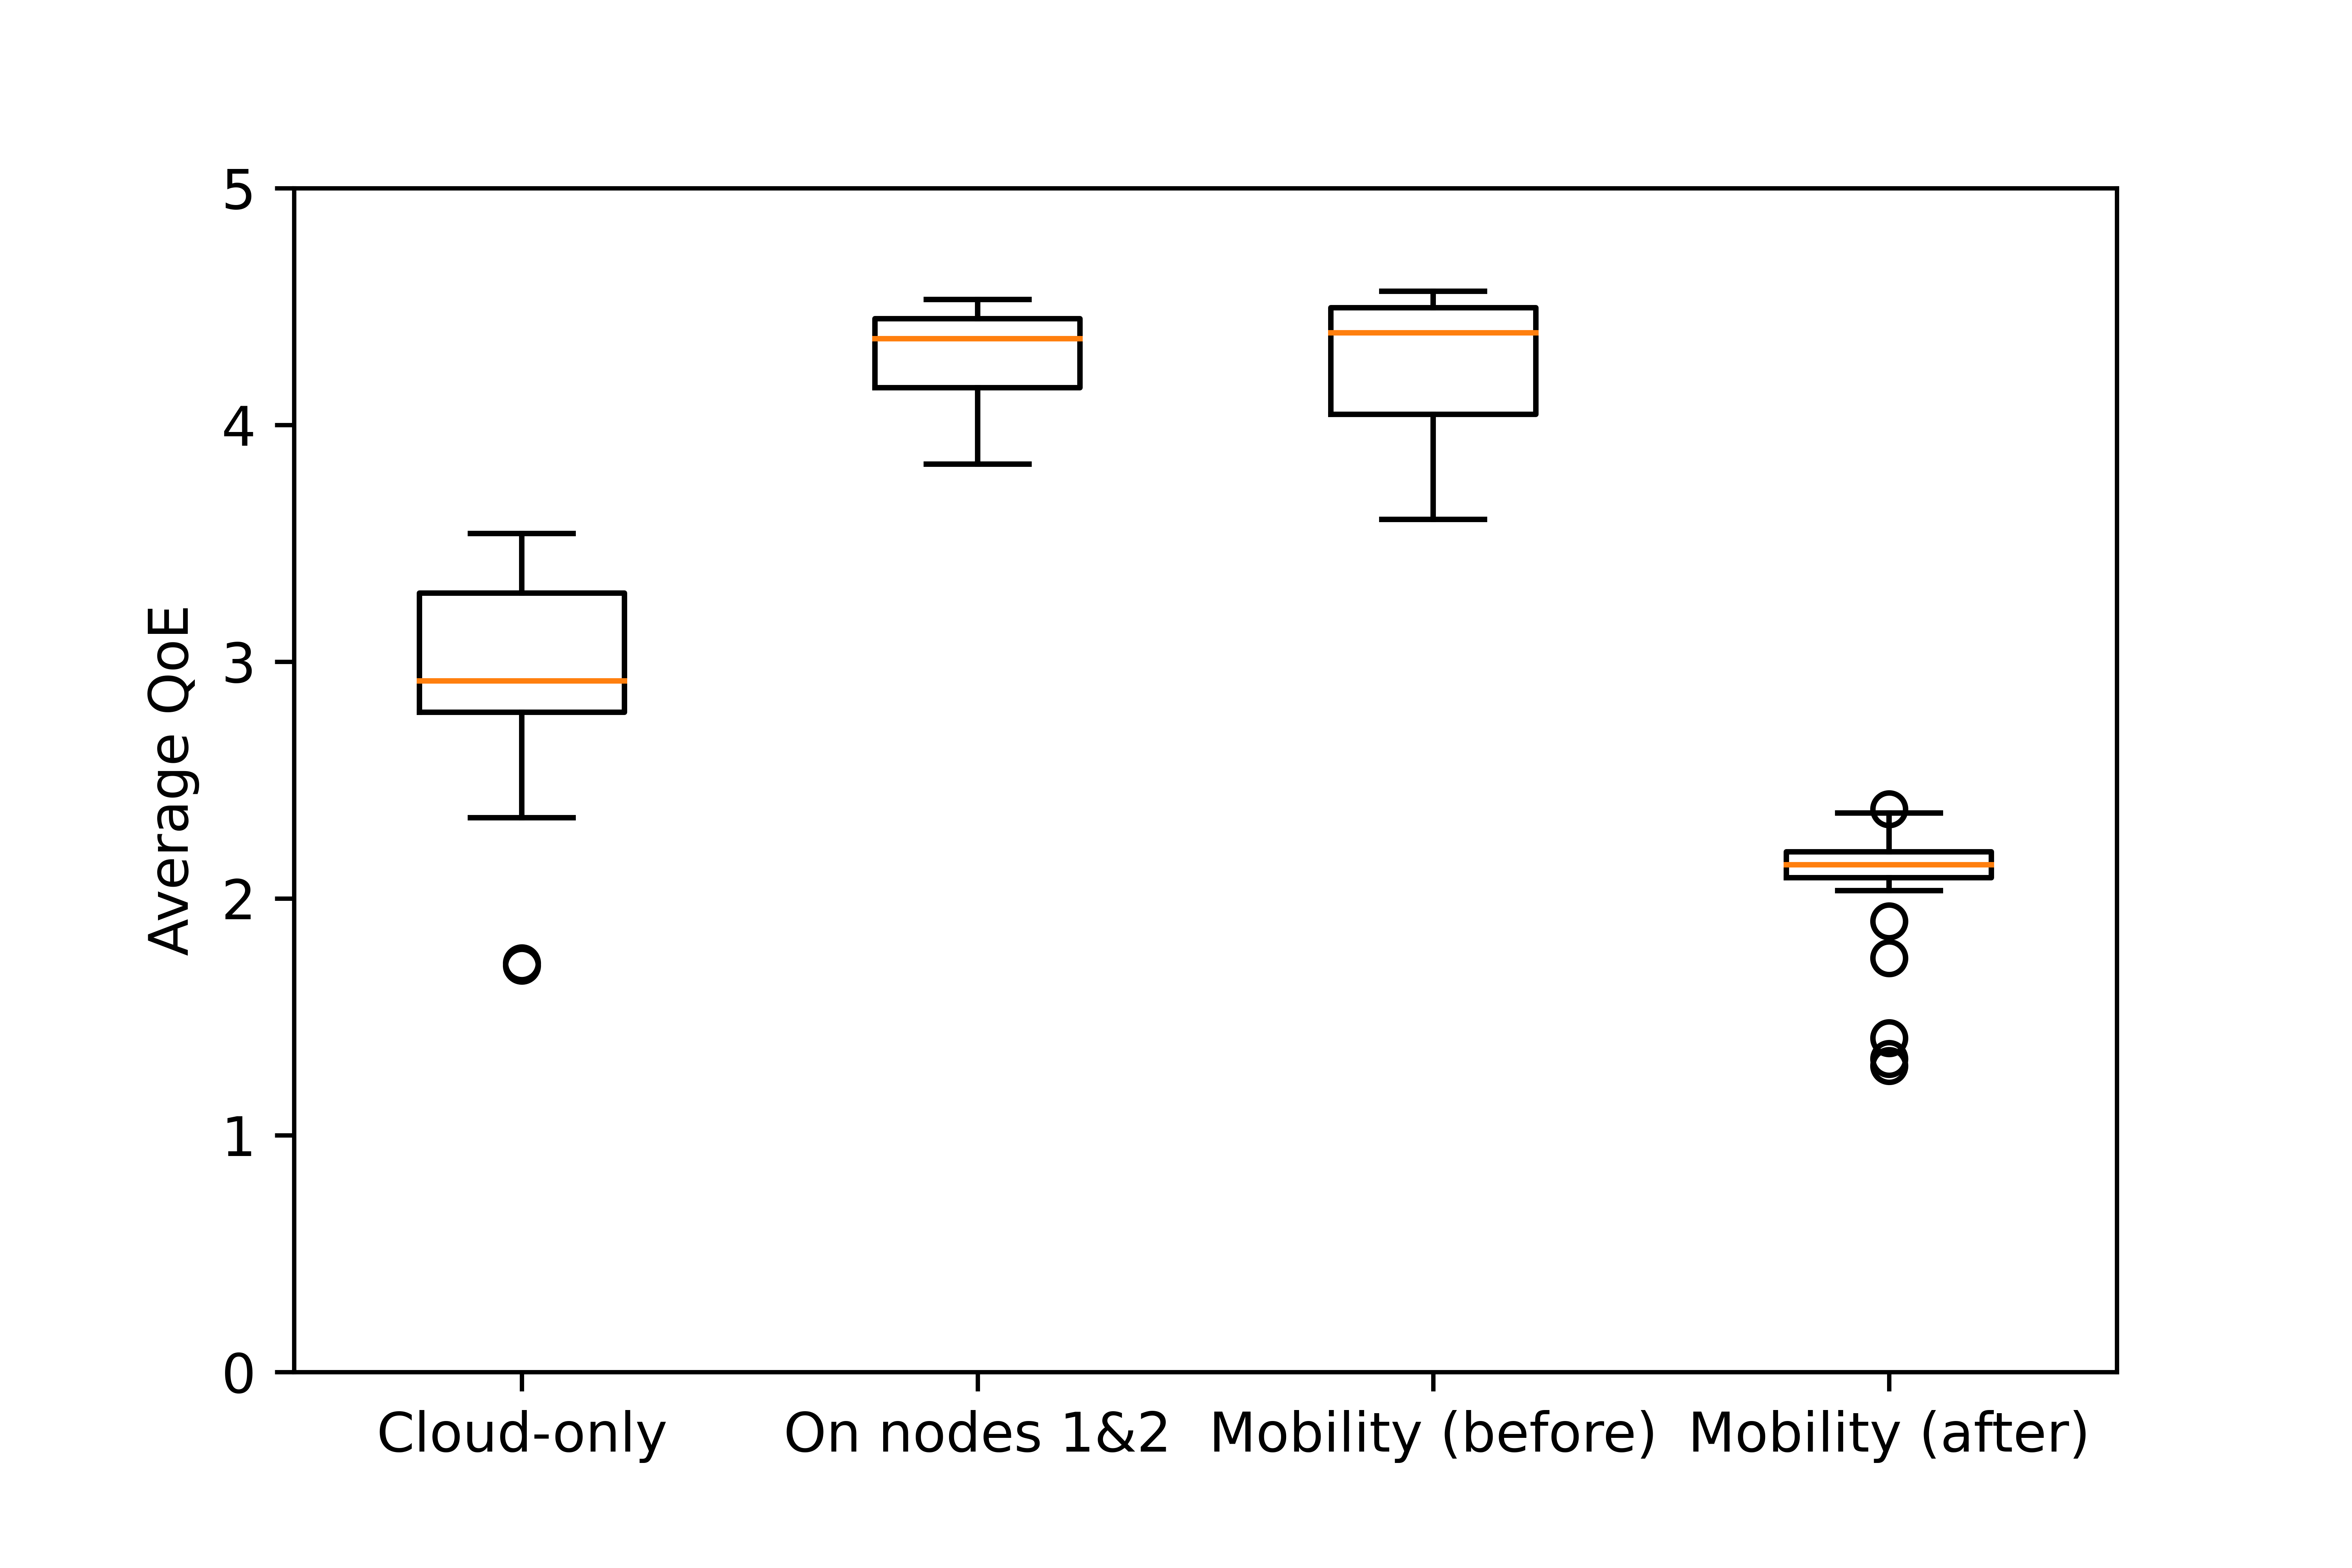
\includegraphics[width=0.31\linewidth]{images/QoEBoxplot-20u.png}
    \label{fig:co-comparison-boxplot}
    }
    \subfigure[]{
    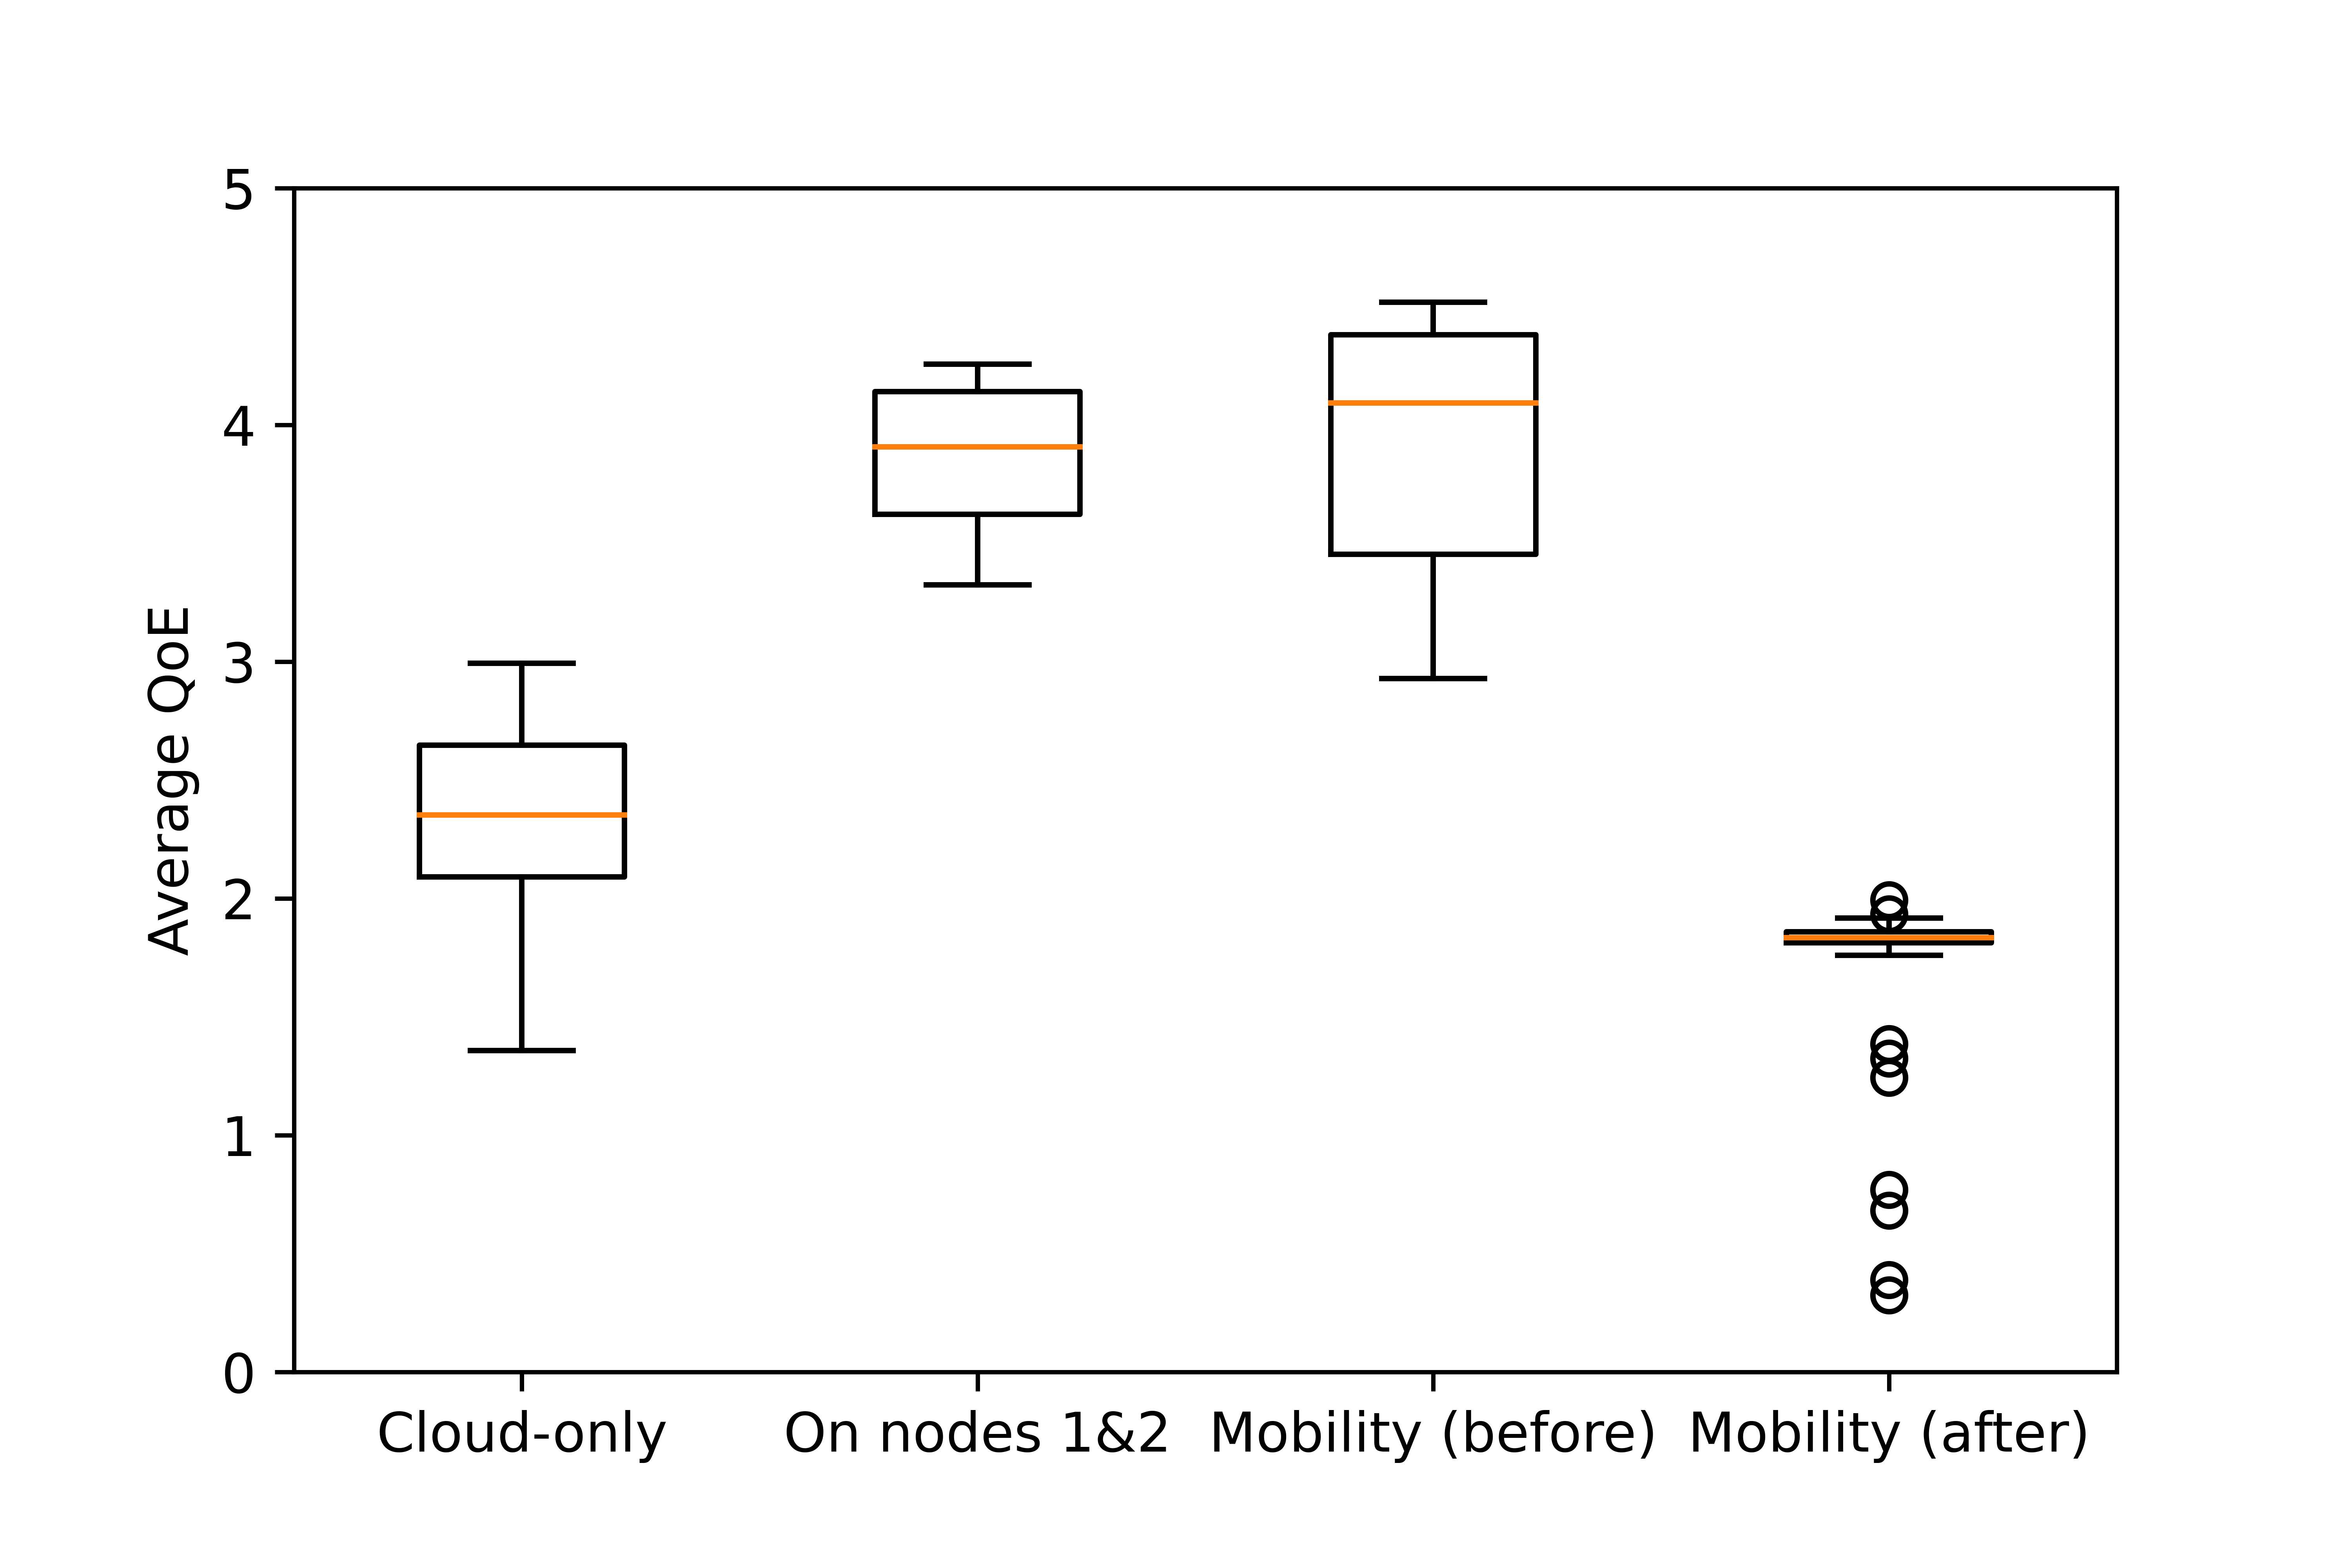
\includegraphics[width=0.31\linewidth]{images/QoEBoxplot-25u.png}
    \label{fig:red-comparison-plot}
    }
    
    \caption{Average QoE results for scenarios with 15, 20 and 25 users per AP.}
    \label{fig:comparison-rof-2}
\end{figure*}


\begin{figure*}
    \centering
    \subfigure[]{
    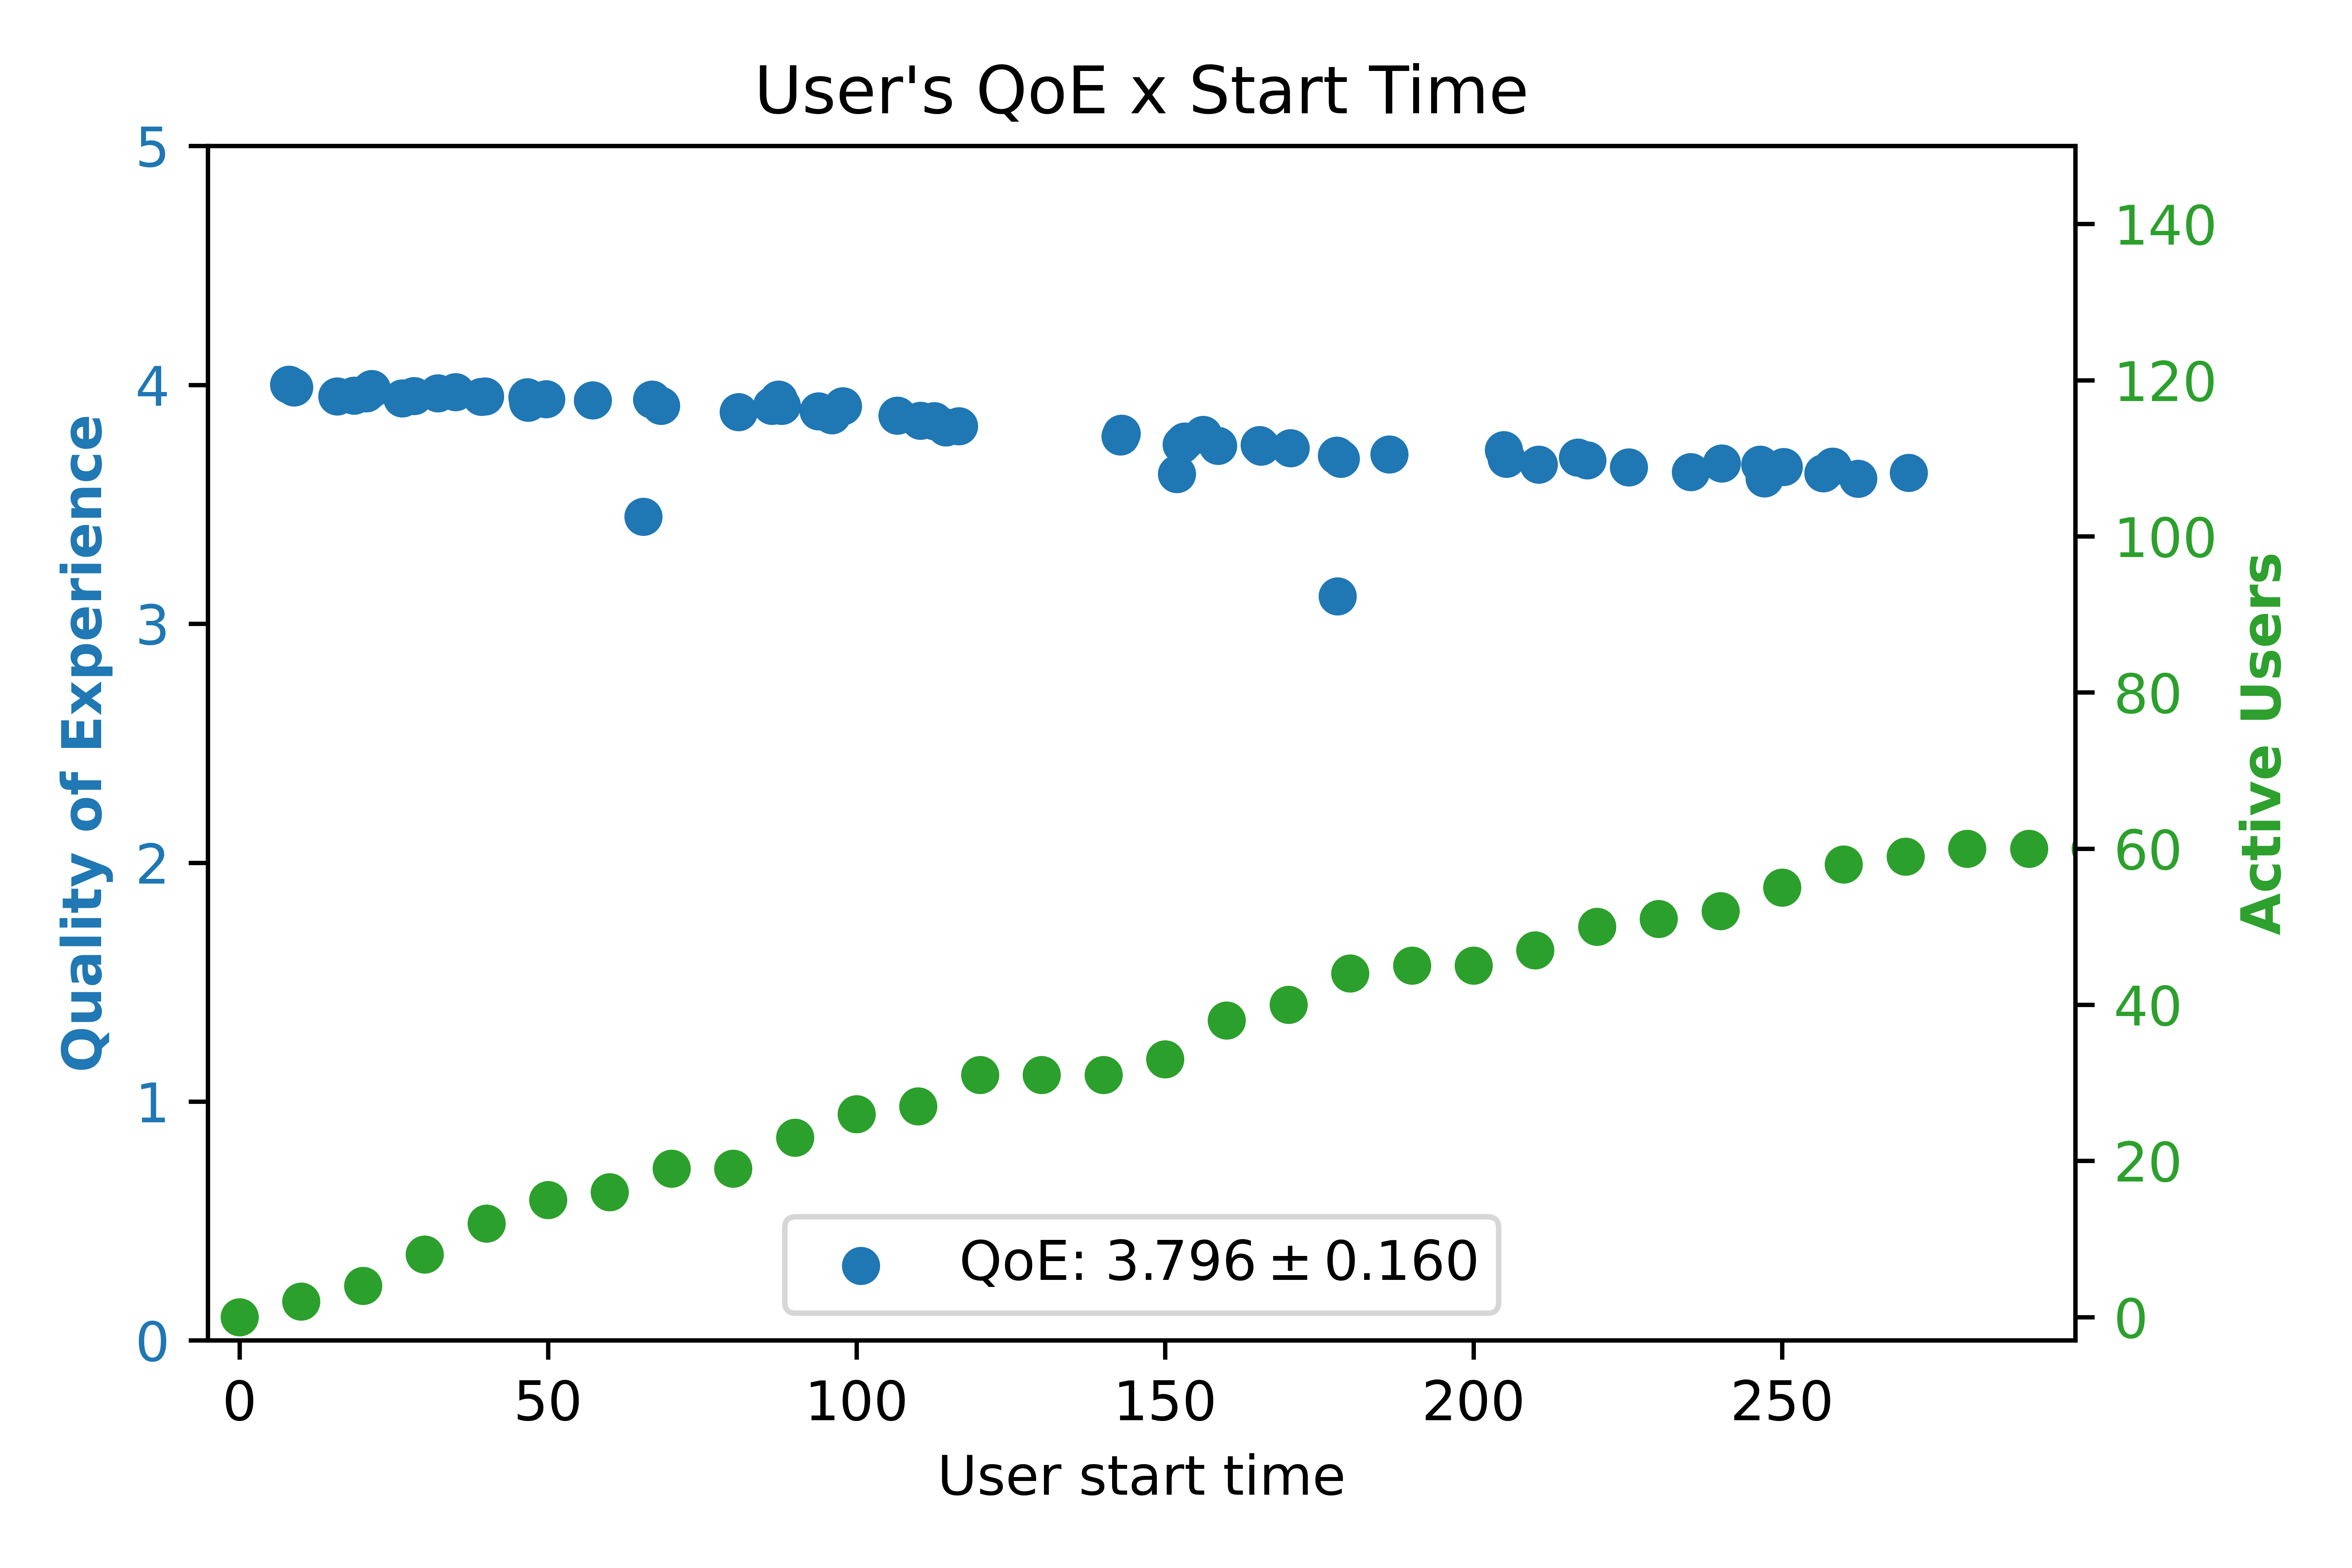
\includegraphics[width=0.31\linewidth]{images/cloud_QoExStartTime15.png}
    \label{fig:rssi-comparison-2}
    }
    \subfigure[]{
    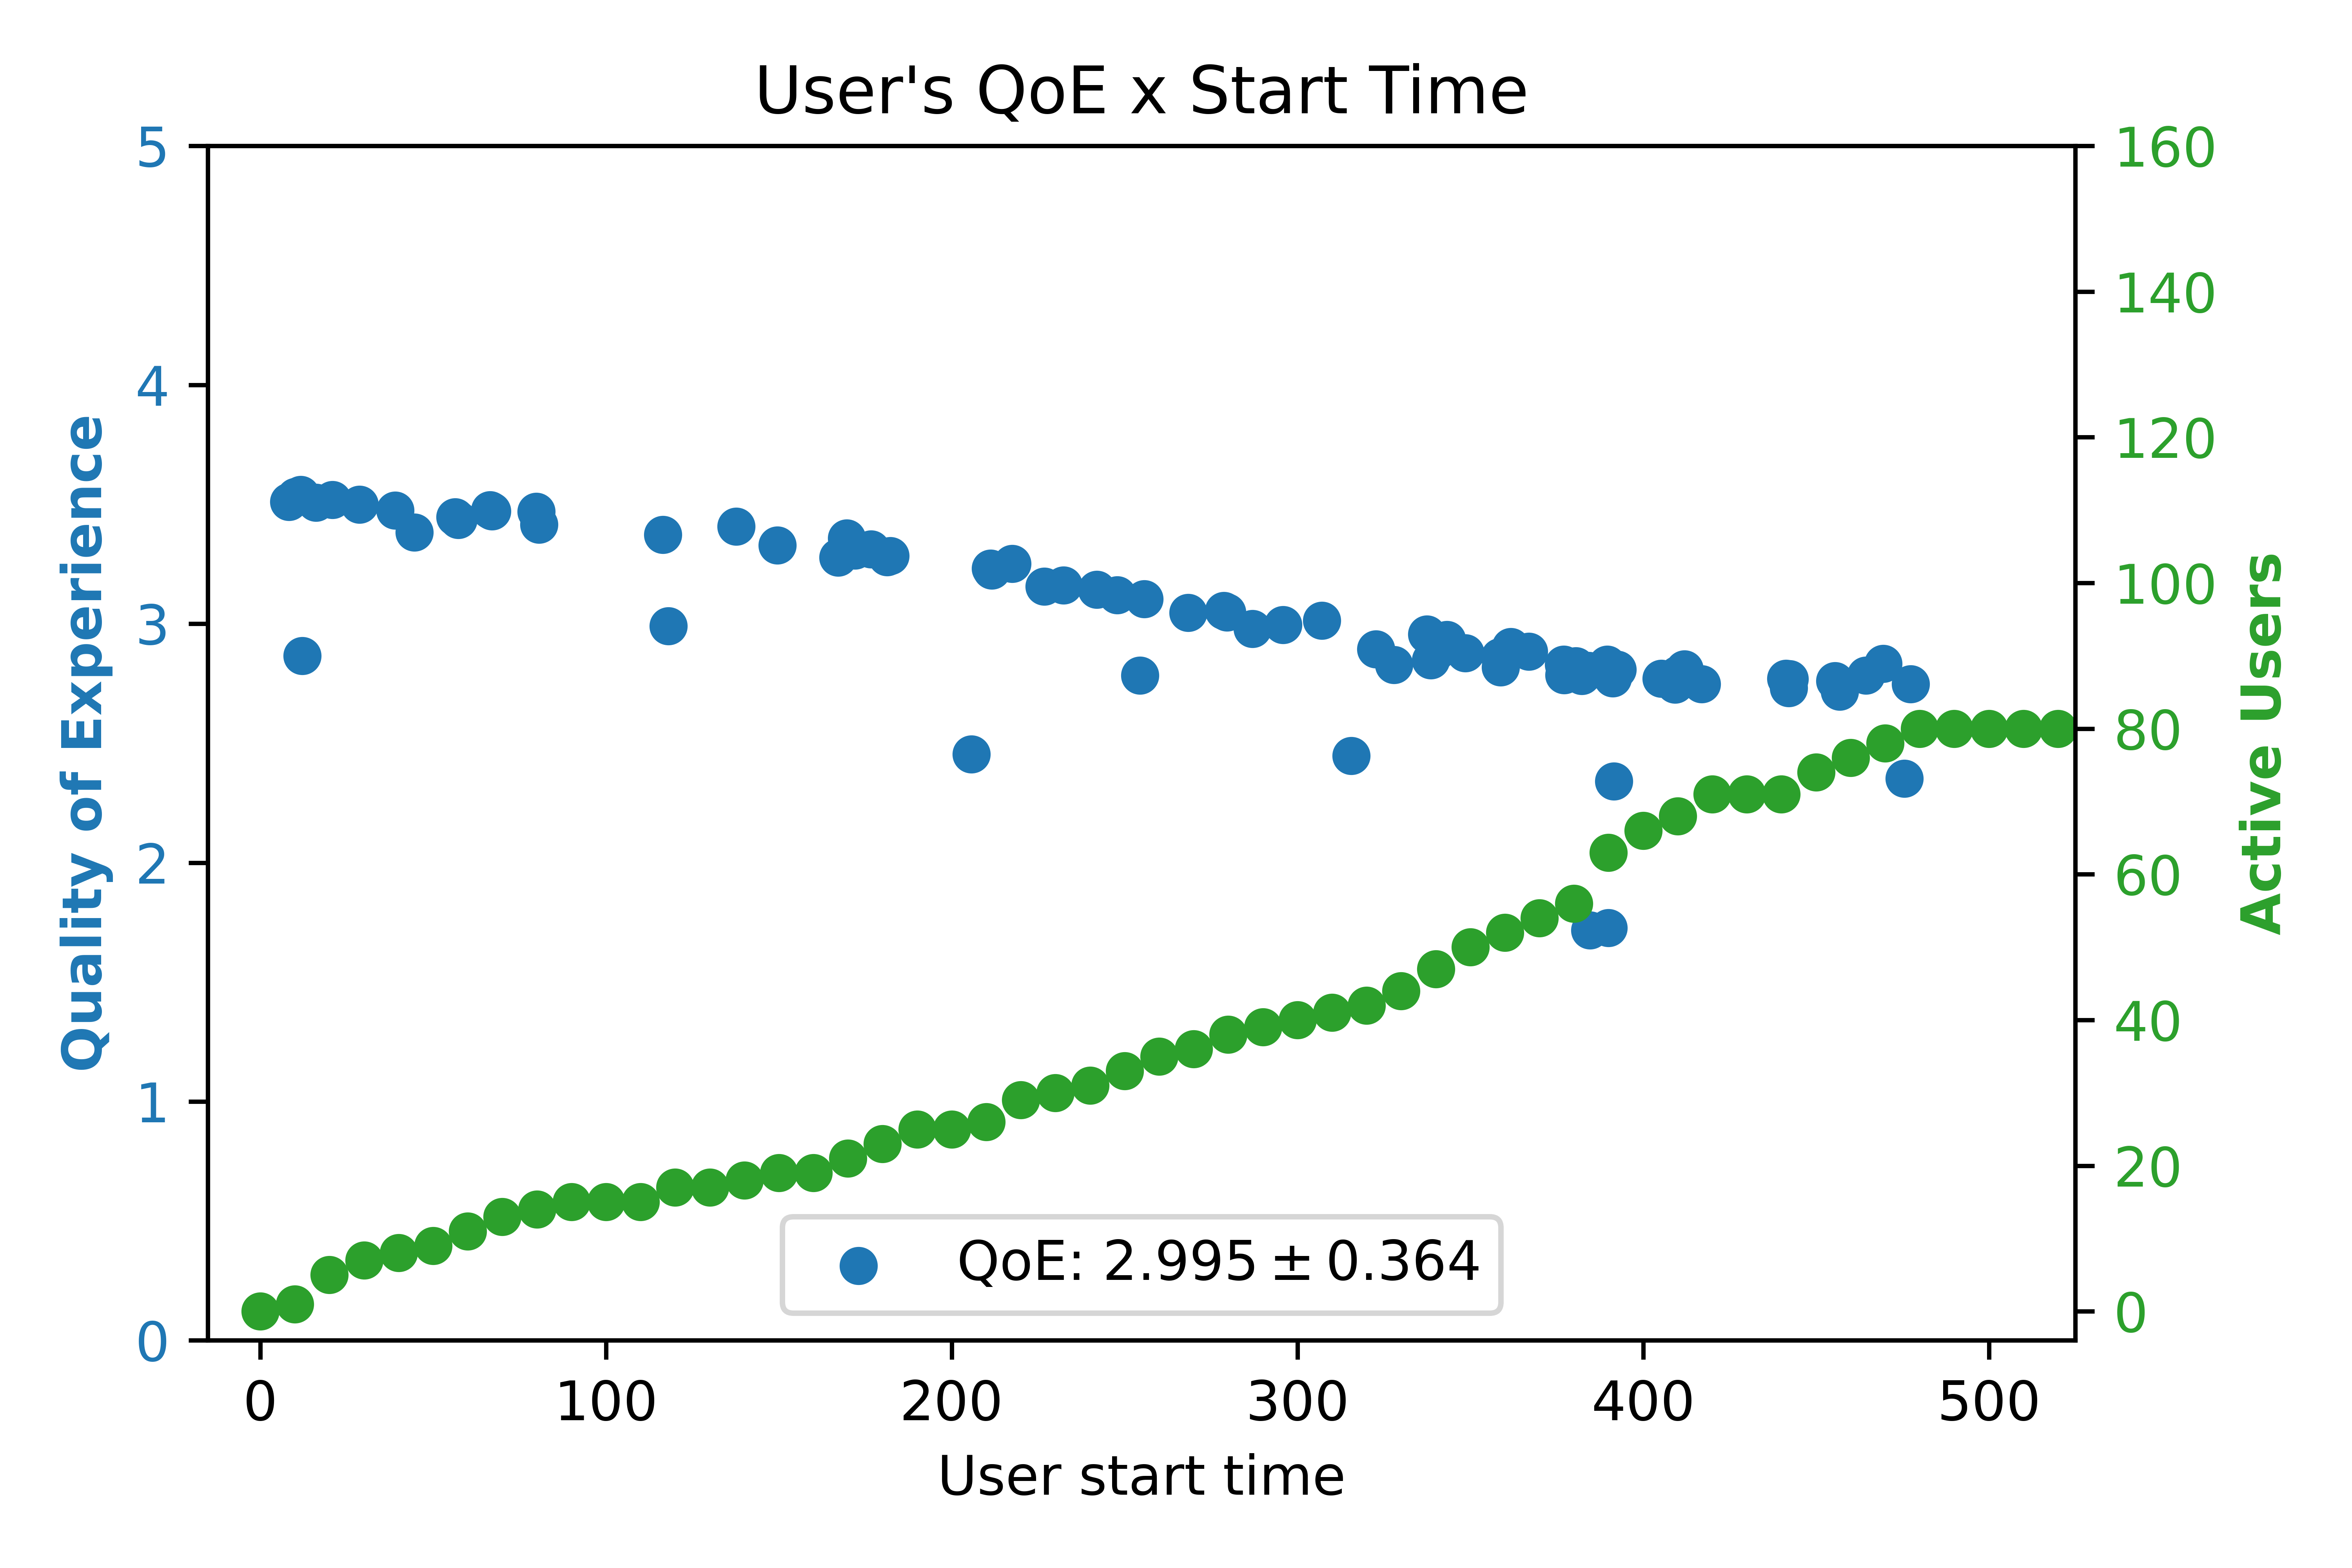
\includegraphics[width=0.31\linewidth]{images/cloud_QoExStartTime20.png}
    \label{fig:plr-comparison-2}
    }
    \subfigure[]{
    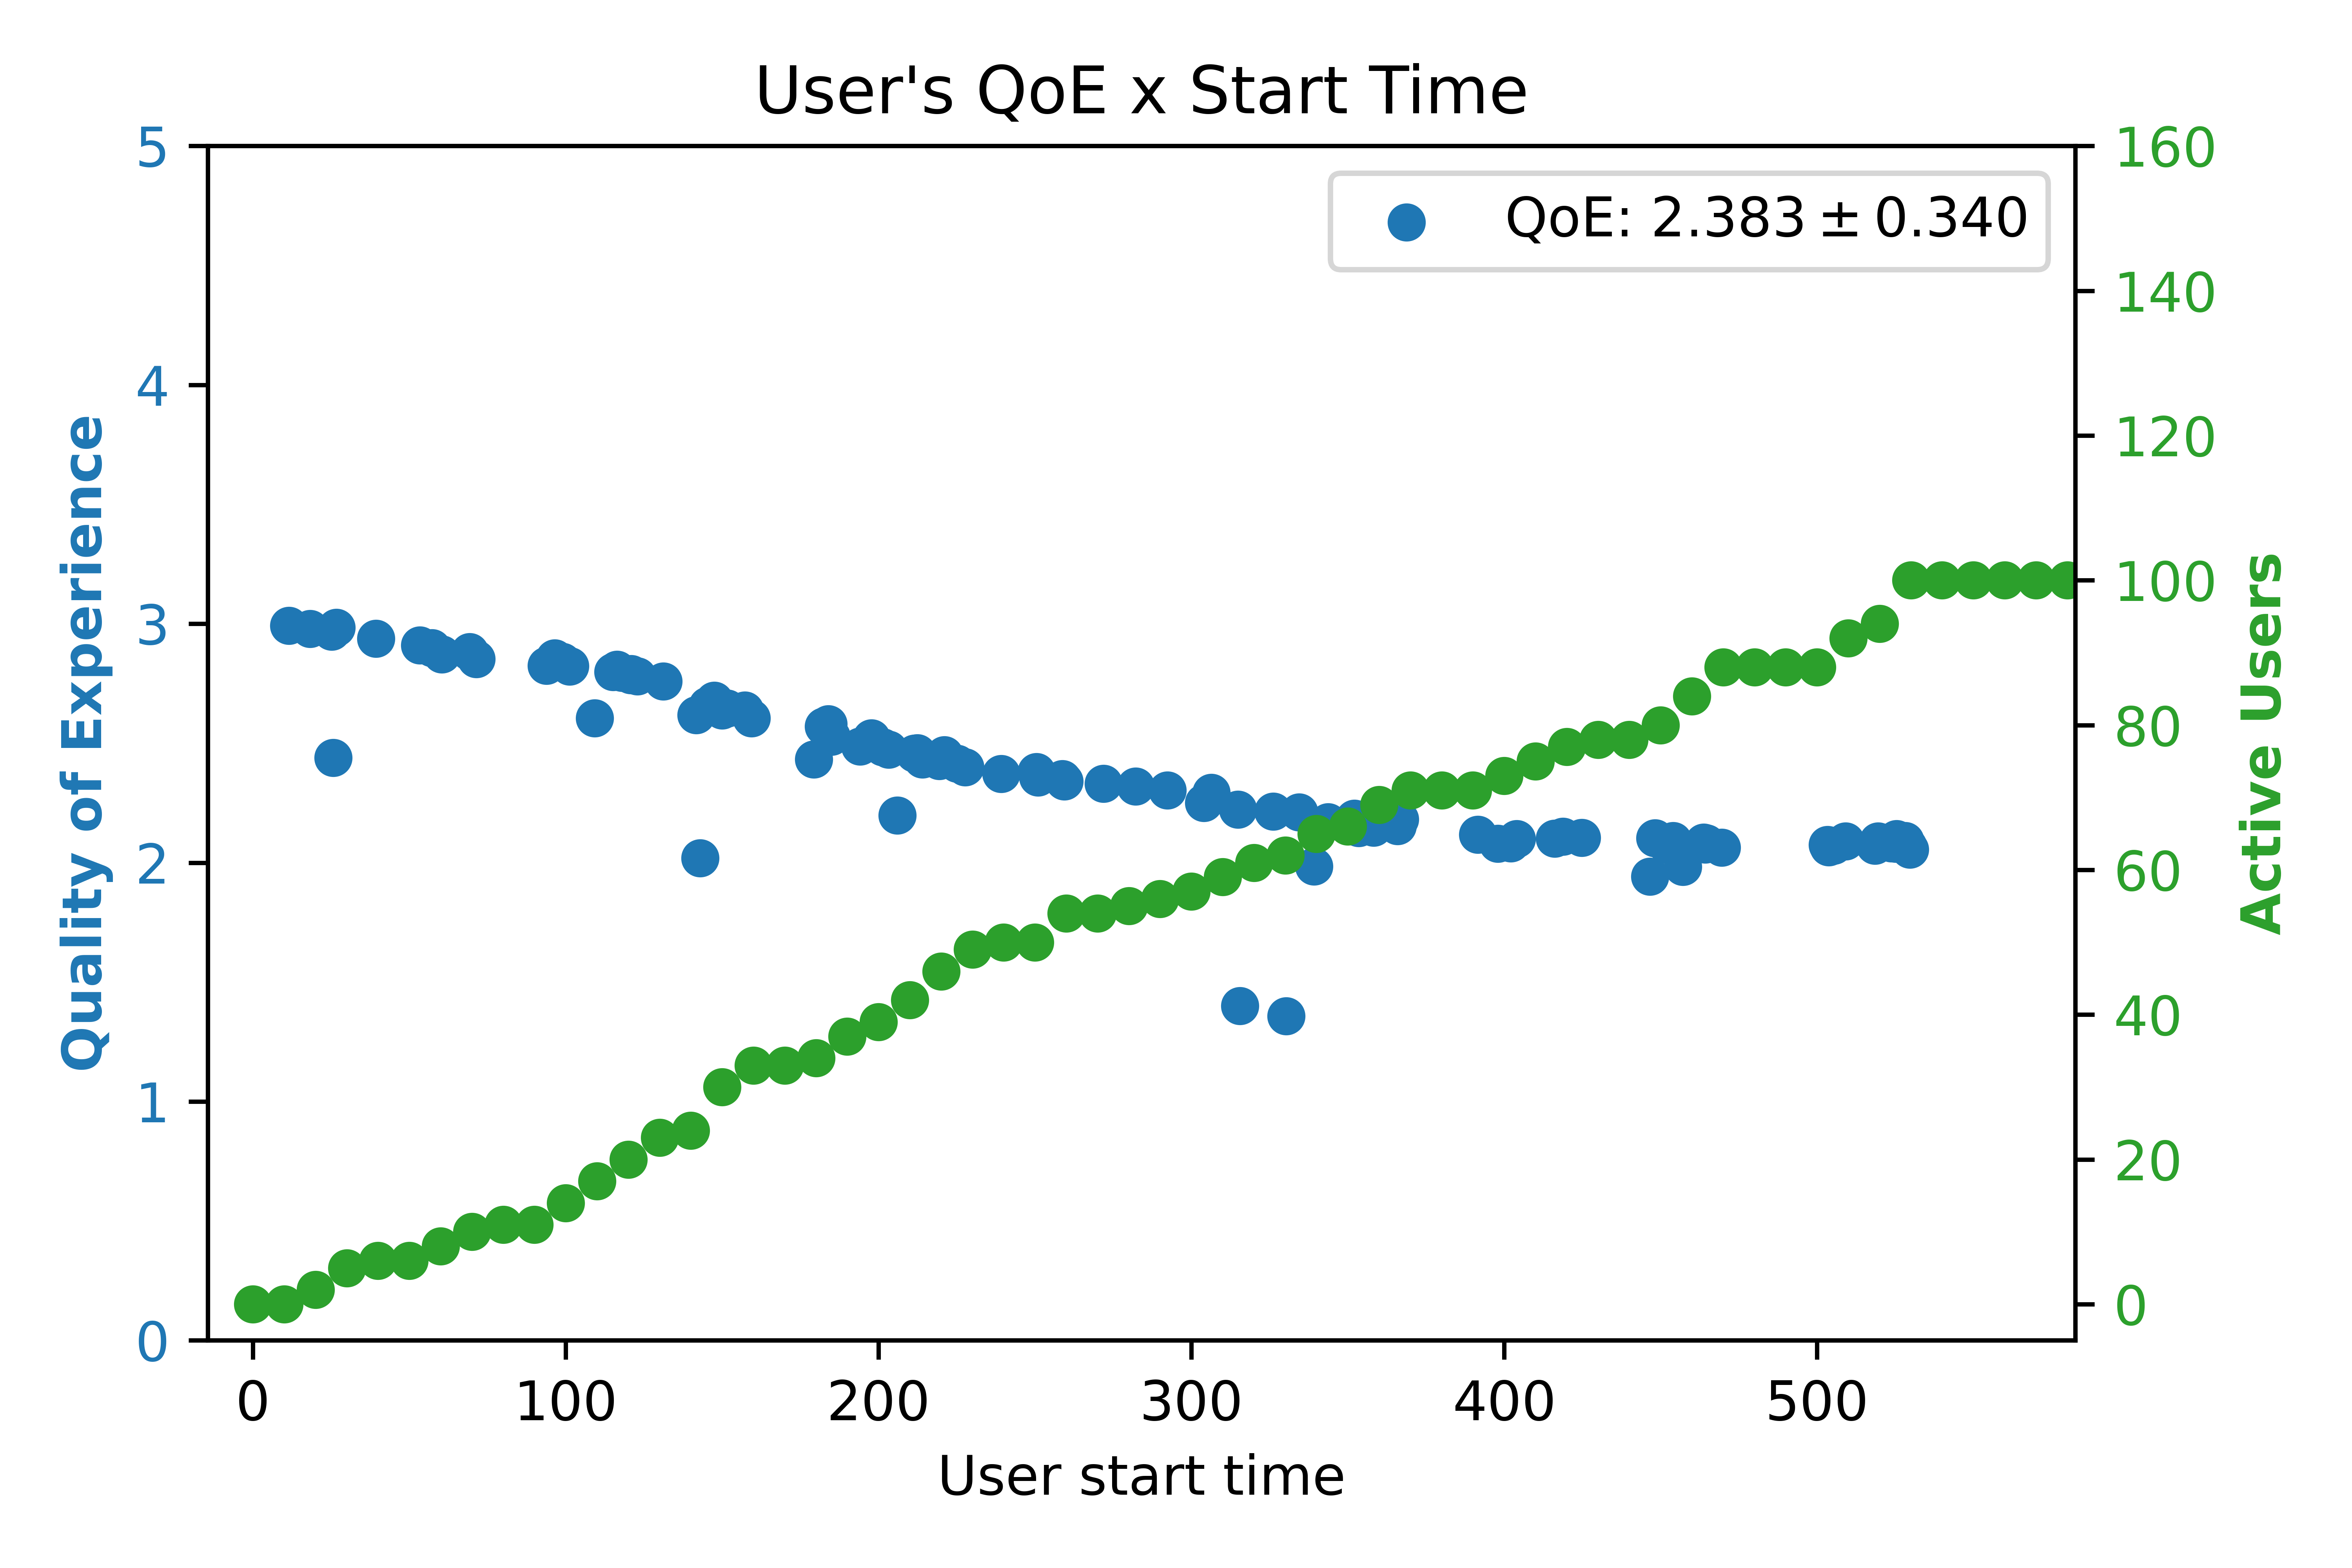
\includegraphics[width=0.31\linewidth]{images/cloud_QoExStartTime25.png}
    \label{fig:plr-comparison-2}
    }
    
    \subfigure[]{
    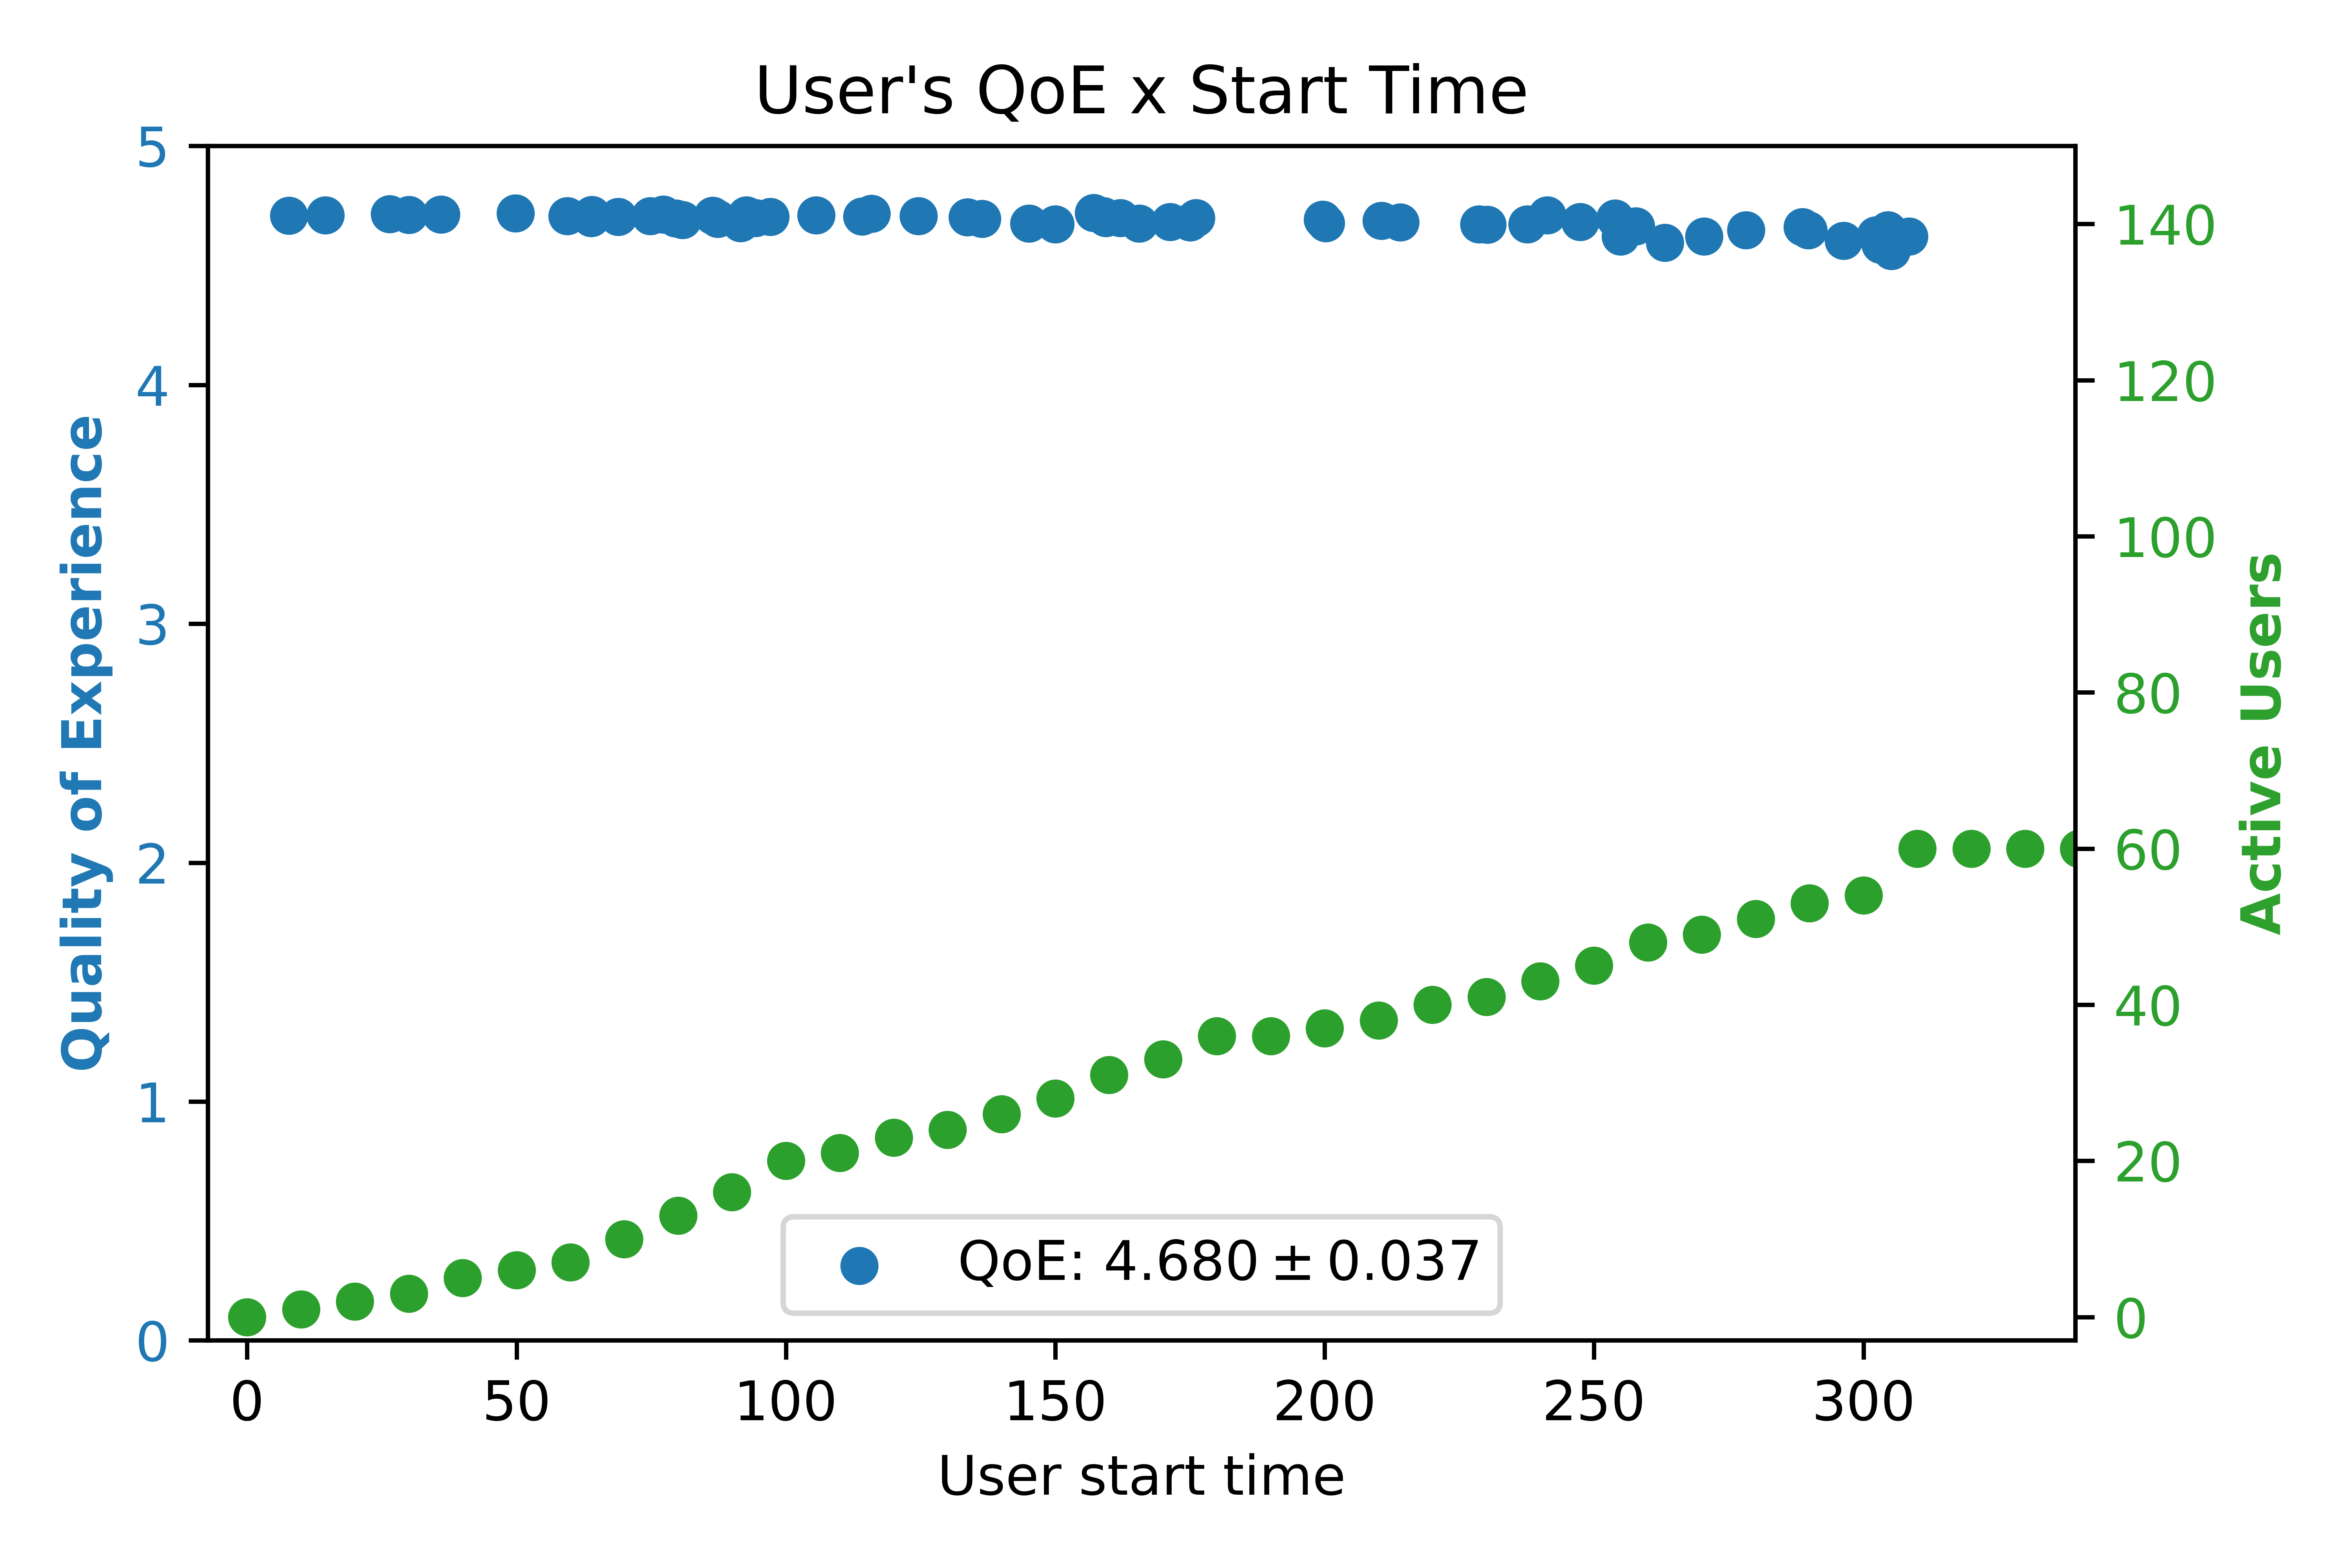
\includegraphics[width=0.31\linewidth]{images/Redicrect_QoExStartTime15.png}
    \label{fig:rssi-comparison-2}
    }
    \subfigure[]{
    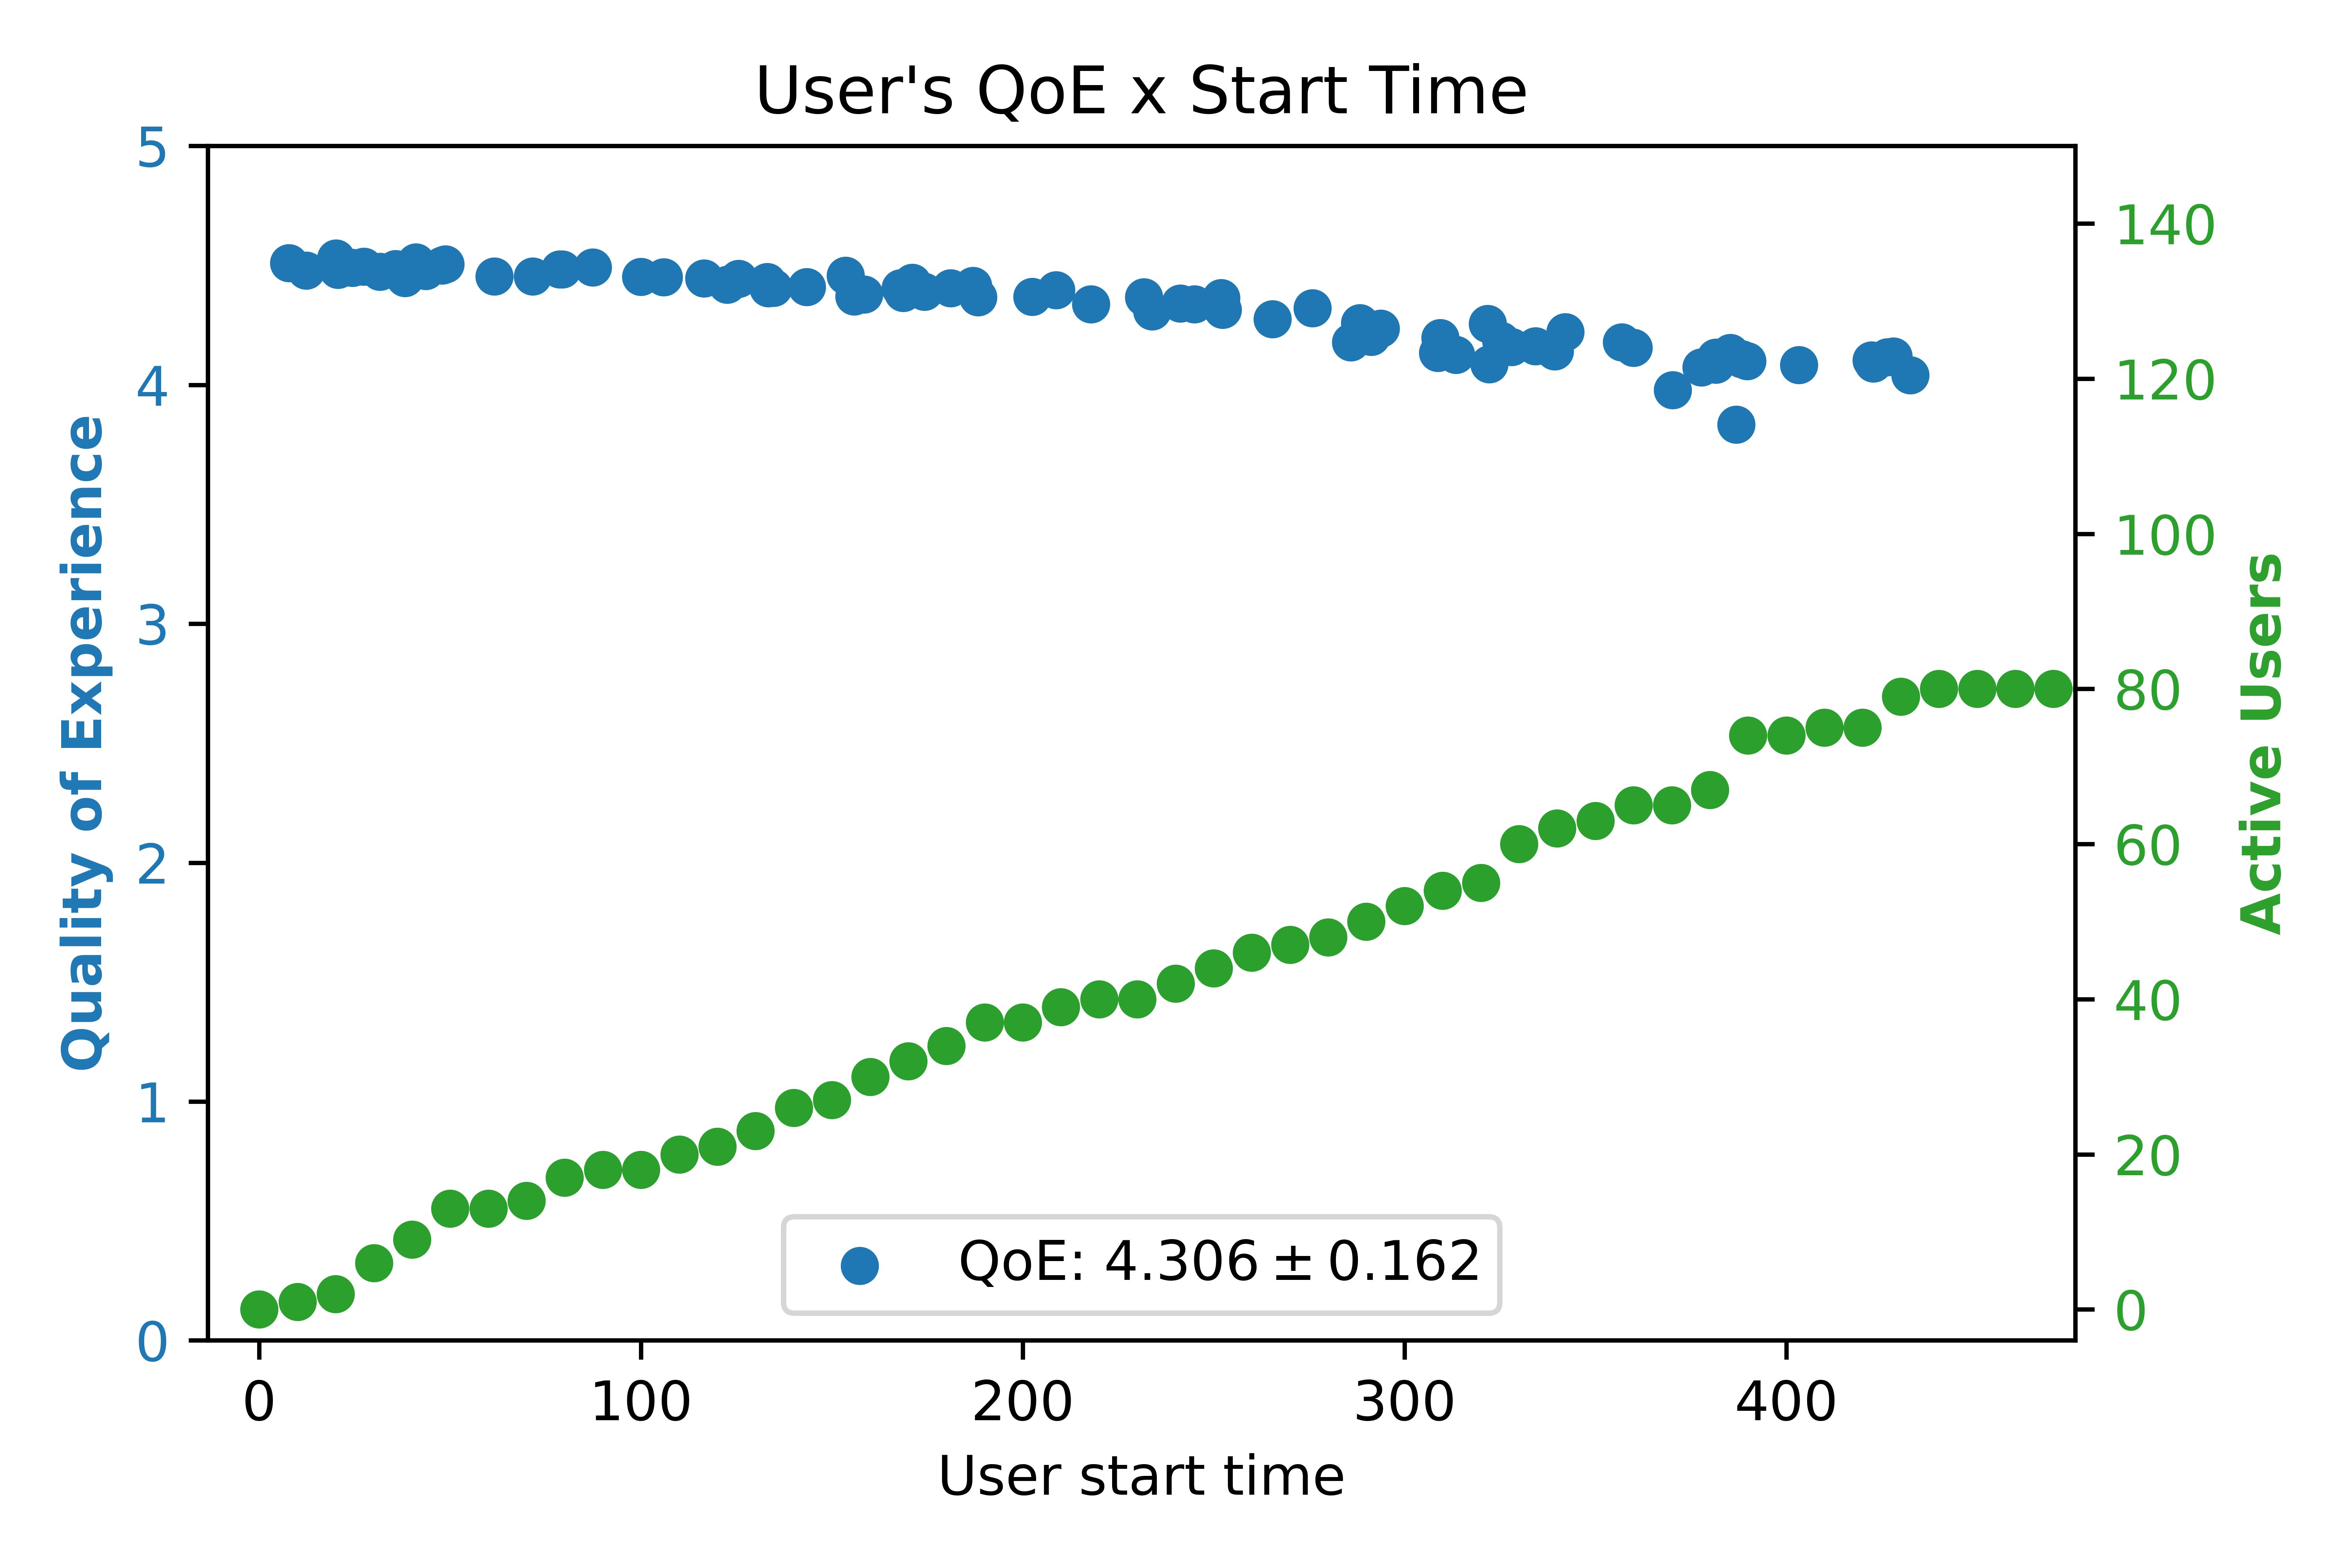
\includegraphics[width=0.31\linewidth]{images/Redicrect_QoExStartTime20.png}
    \label{fig:plr-comparison-2}
    }
    \subfigure[]{
    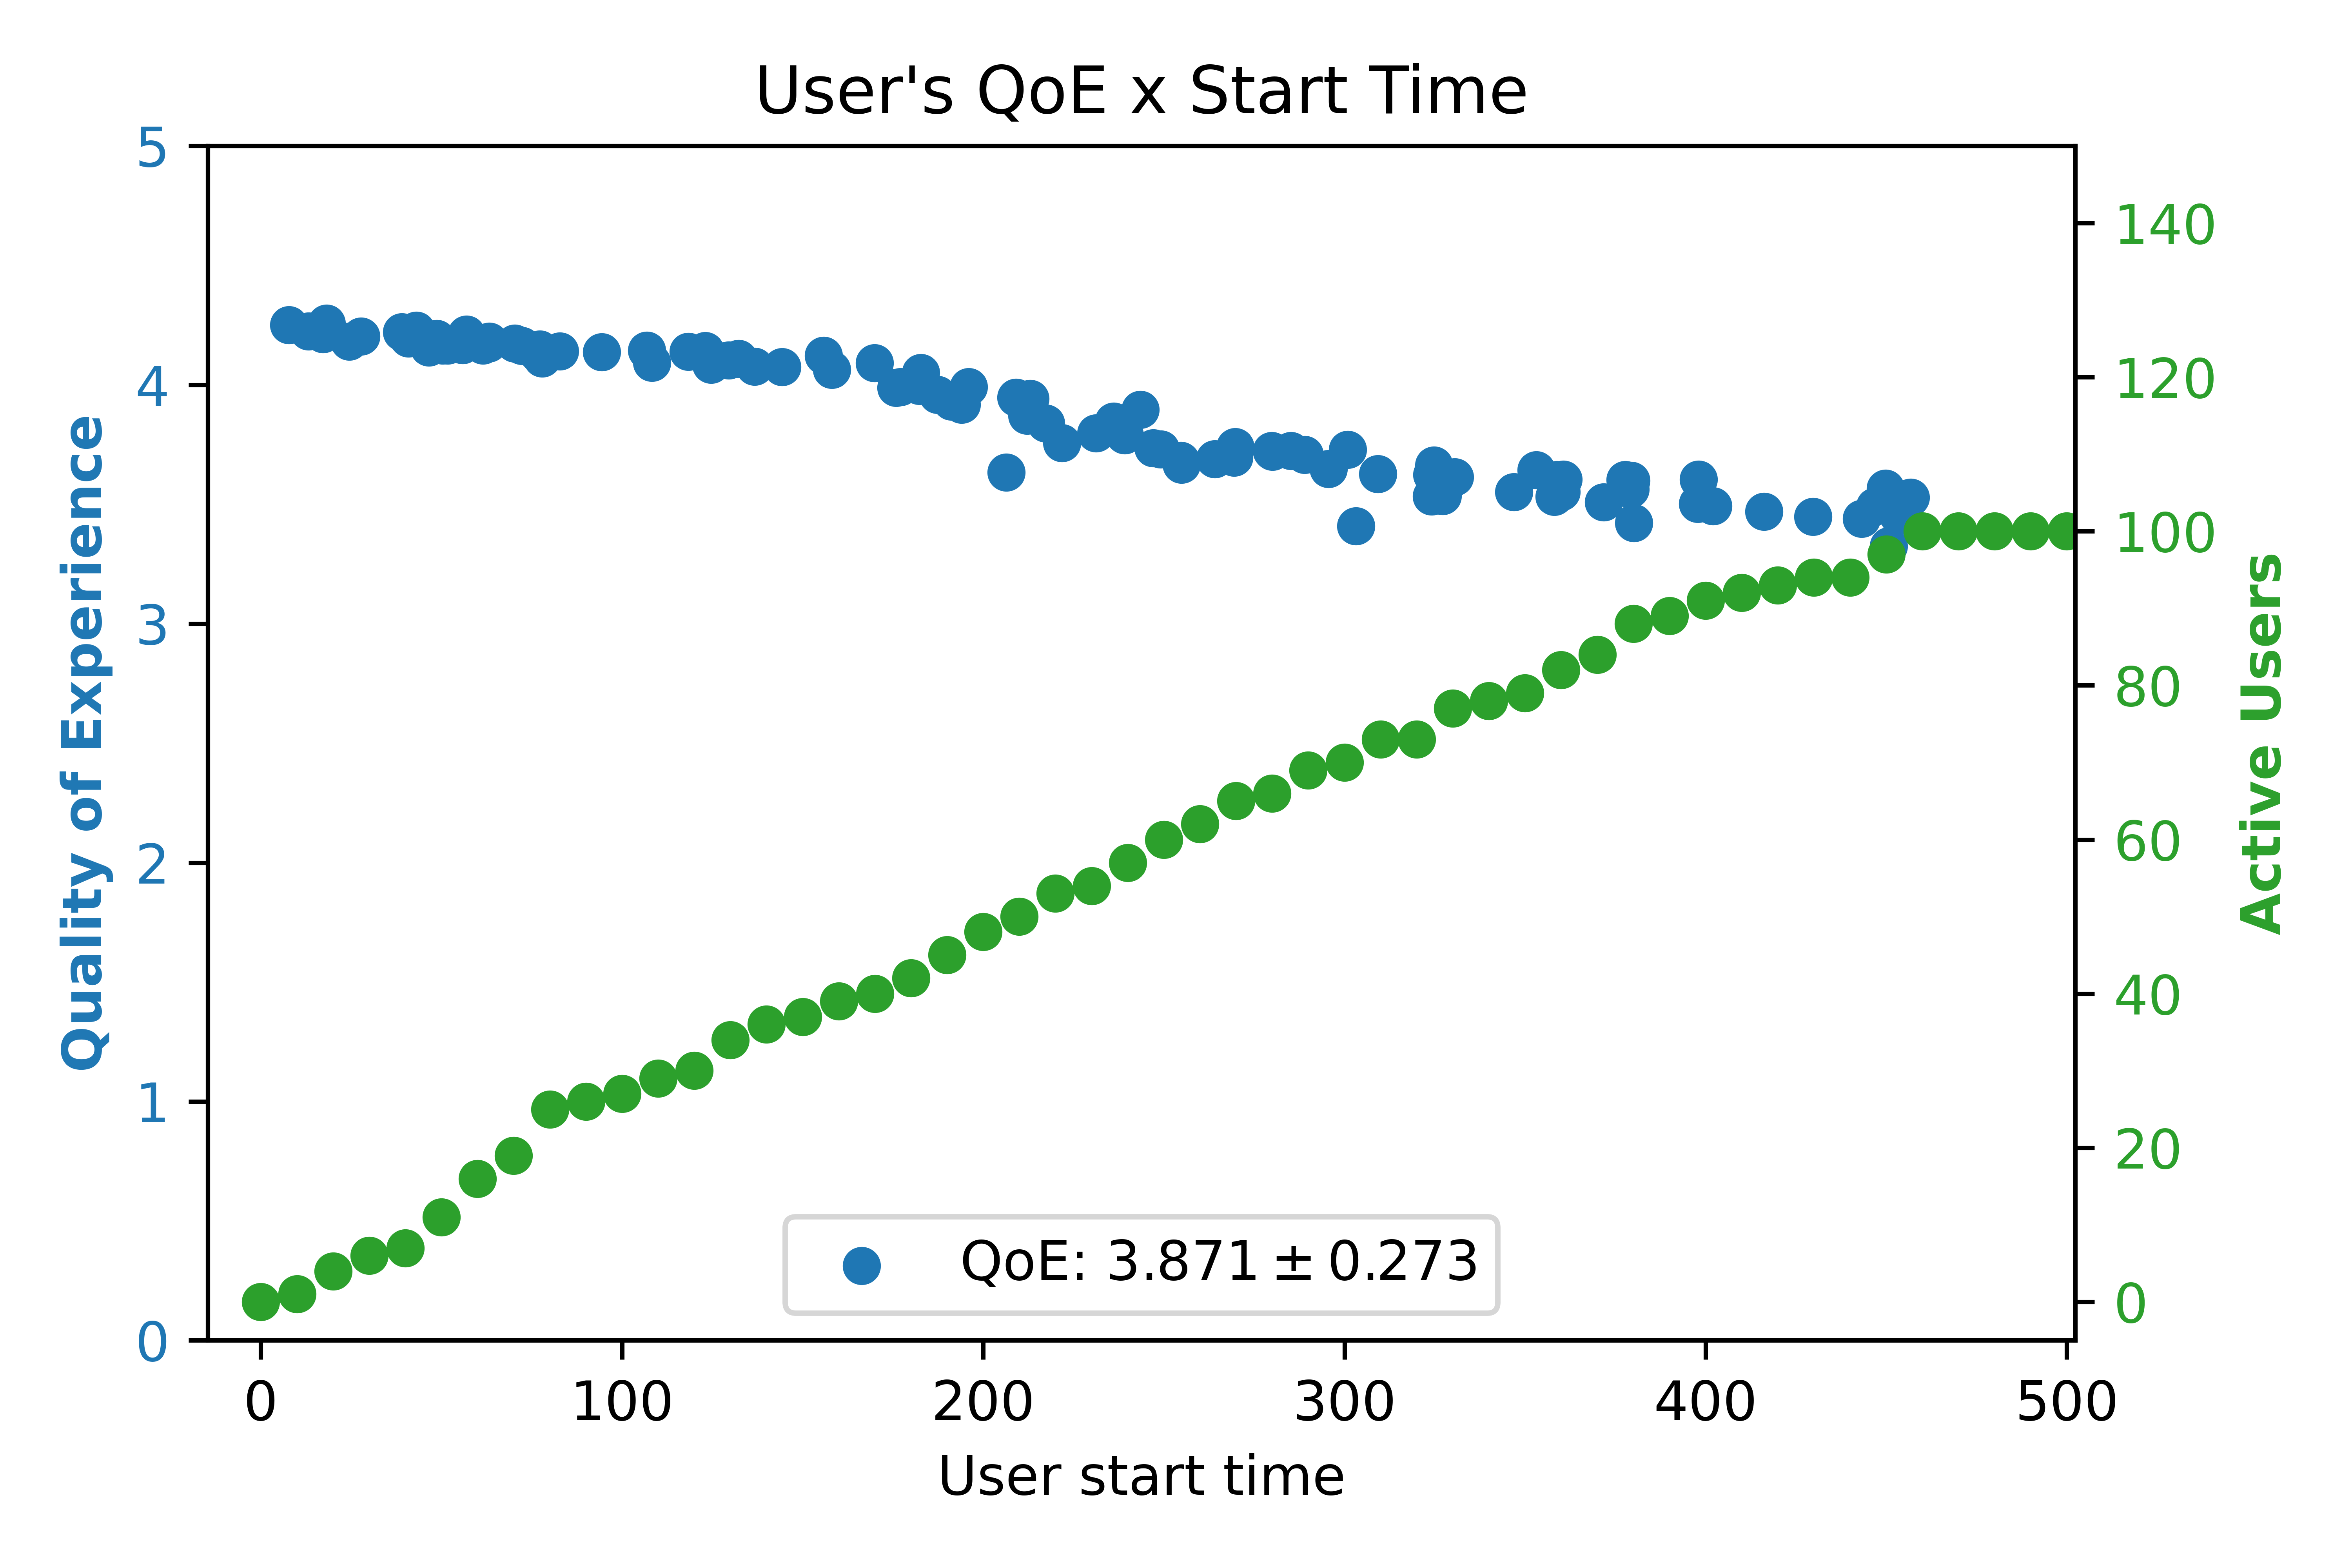
\includegraphics[width=0.31\linewidth]{images/Redicrect_QoExStartTime25.png}
    \label{fig:plr-comparison-2}
    }
    
    \caption{Impact of system on the network performance. Distance \textit{d} between sensor node and antennas of 8m in a semi-NLOS scenario.}
    \label{fig:comparison-qoe-2}
\end{figure*}

\subsection{Results}

We made the experiment illustrated in Figure~\ref{fig:red-comparison-plot} to show the average QoE as shown in~\ref{qoe-equation} to 15, 20 and 25 users. In this experiment, a medida que os usuários vão chegando o QoE final tenda a ser um pouco menor do que o anterior 